\documentclass[14pt]{beamer}
\usepackage[utf8]{inputenc}
\usepackage[ngerman]{babel}
\usepackage{amsmath}
\usepackage{amsfonts}
\usepackage{amssymb}
\usepackage{color}
\usetheme{default}
\usepackage{tikz}
\usetikzlibrary{decorations.text}
\usepackage{slashed}
\usepackage{multimedia}
\usepackage{textpos}

\usepackage{graphics}
\graphicspath{{images/}}

\setbeamercolor{normal text}{fg=white}
\setbeamercolor{frametitle}{fg=white}
\usebeamercolor[fg]{normal text}

\newcommand{\arcsegment}[7]{
	\def\innerRadius{#1};
	\def\outerRadius{#2};
	\def\startAngle{#3}
	\def\widthAngle{#4};
	\def\myfillcolor{#5};
	\filldraw<#7->[fill=\myfillcolor!20!white, draw=\myfillcolor!50!black] (\startAngle:\innerRadius) -- (\startAngle:\outerRadius) arc (\startAngle:\startAngle+\widthAngle:\outerRadius) -- (\startAngle+\widthAngle:\innerRadius) arc (\startAngle+\widthAngle:\startAngle:\innerRadius);
	\path<#7->[] decorate [decoration={text along path, text={|\small|#6}, text align = {align = center}, raise = -1.0ex}] { (\startAngle+\widthAngle:\outerRadius/2+\innerRadius/2) arc (\startAngle+\widthAngle:\startAngle:\outerRadius/2+\innerRadius/2)};
}

\newcommand{\arcsegmenttwo}[7]{
	\def\innerRadius{#1};
	\def\outerRadius{#2};
	\def\startAngle{#3}
	\def\widthAngle{#4};
	\def\myfillcolor{#5};
	\filldraw<#7->[fill=\myfillcolor, draw=black] (\startAngle:\innerRadius) -- (\startAngle:\outerRadius) arc (\startAngle:\startAngle+\widthAngle:\outerRadius) -- (\startAngle+\widthAngle:\innerRadius) arc (\startAngle+\widthAngle:\startAngle:\innerRadius);
	\path<#7->[] decorate [decoration={text along path, text={|\small|#6}, text align = {align = center}, raise = -1.0ex}] { (\startAngle+\widthAngle:\outerRadius/2+\innerRadius/2) arc (\startAngle+\widthAngle:\startAngle:\outerRadius/2+\innerRadius/2)};
}

\begin{document}
\usebackgroundtemplate{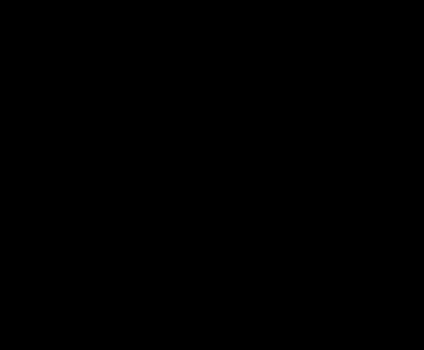
\includegraphics[width=\paperwidth]{black.png}}%
	\author{Thomas Keck}
	\title{Die Welt jenseits \\von $10^{-16}$ bis $10^{24}$ Metern}
	\frame[plain]{\maketitle}
	
	\usebackgroundtemplate{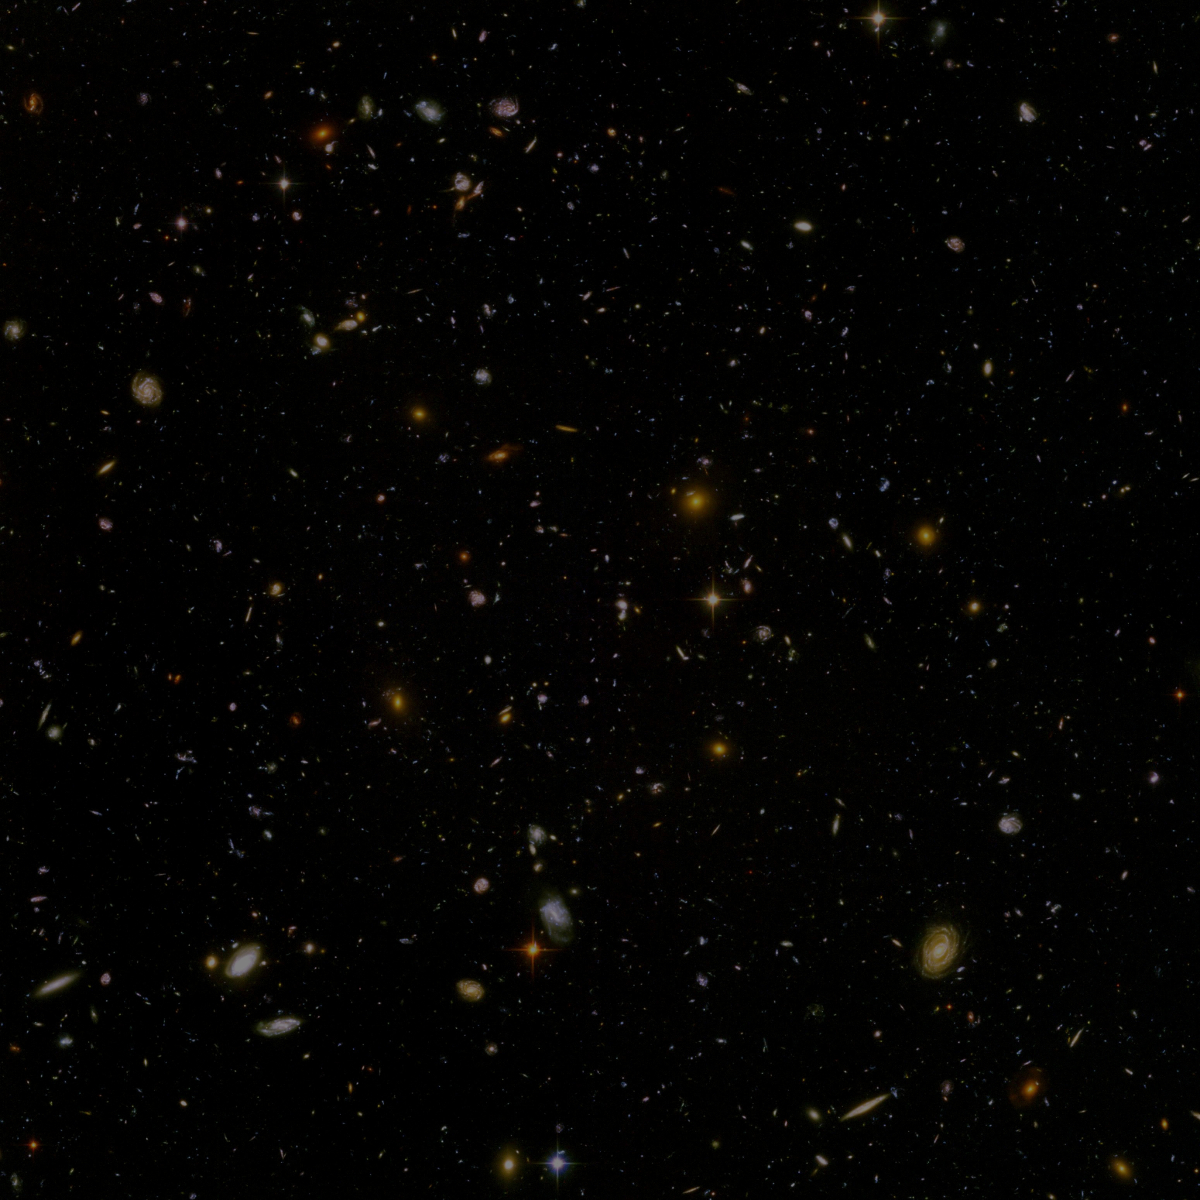
\includegraphics[width=\paperwidth]{hubble.jpg}}
	\begin{frame}
		\centering
		\huge{Powers of Ten -- Teil I}
	\end{frame}

\begin{frame}
	\centering
	\huge{Der Urknall}
\end{frame}

\begin{frame}{Planck}
	\begin{center}
		\begin{tikzpicture}
			\node at (5.5,-2) {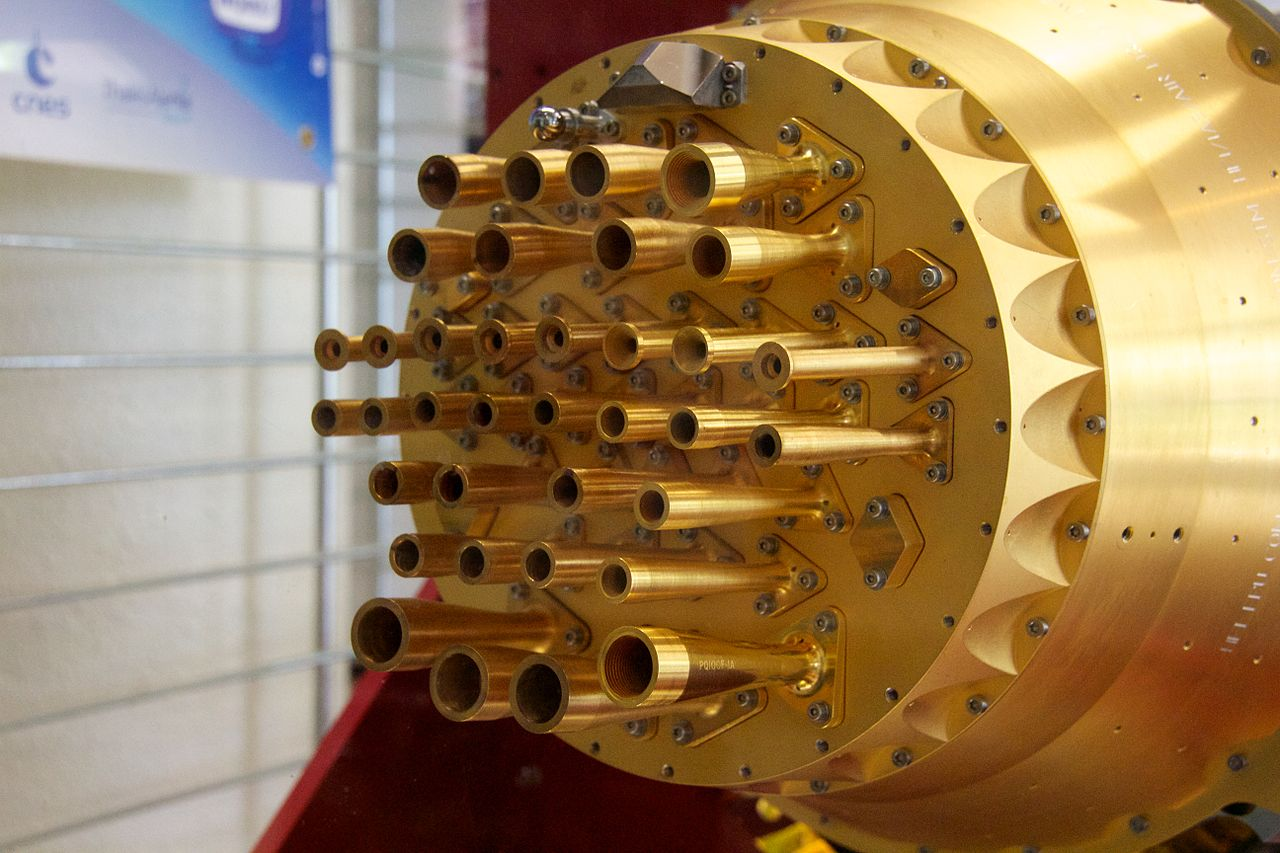
\includegraphics[width=0.45\textwidth]{1280px-Planck_HFI_qualification_model_5.jpg}};
			\node at (5.5,2) {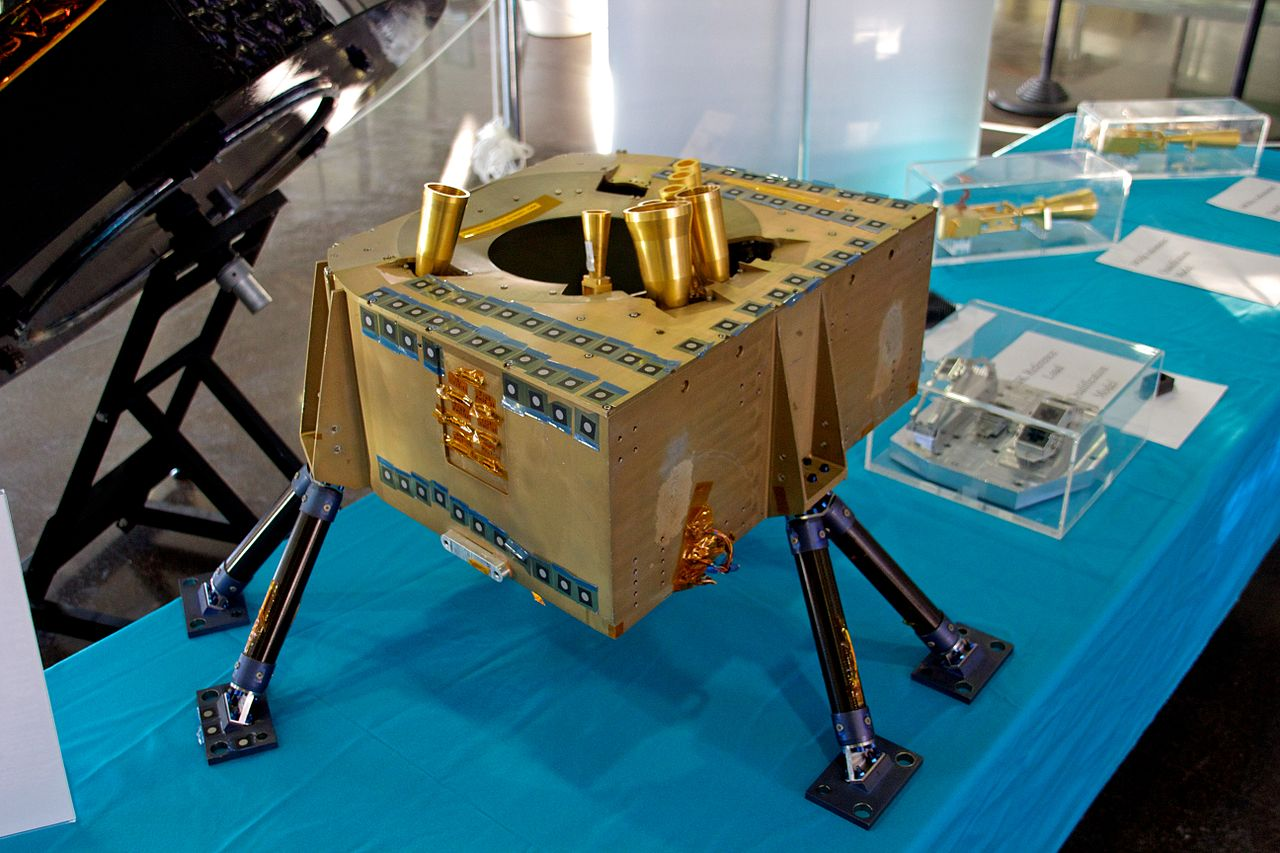
\includegraphics[width=0.45\textwidth]{1280px-Planck_LFI_focal_plane_model.jpg}};
			\node at (0,0) {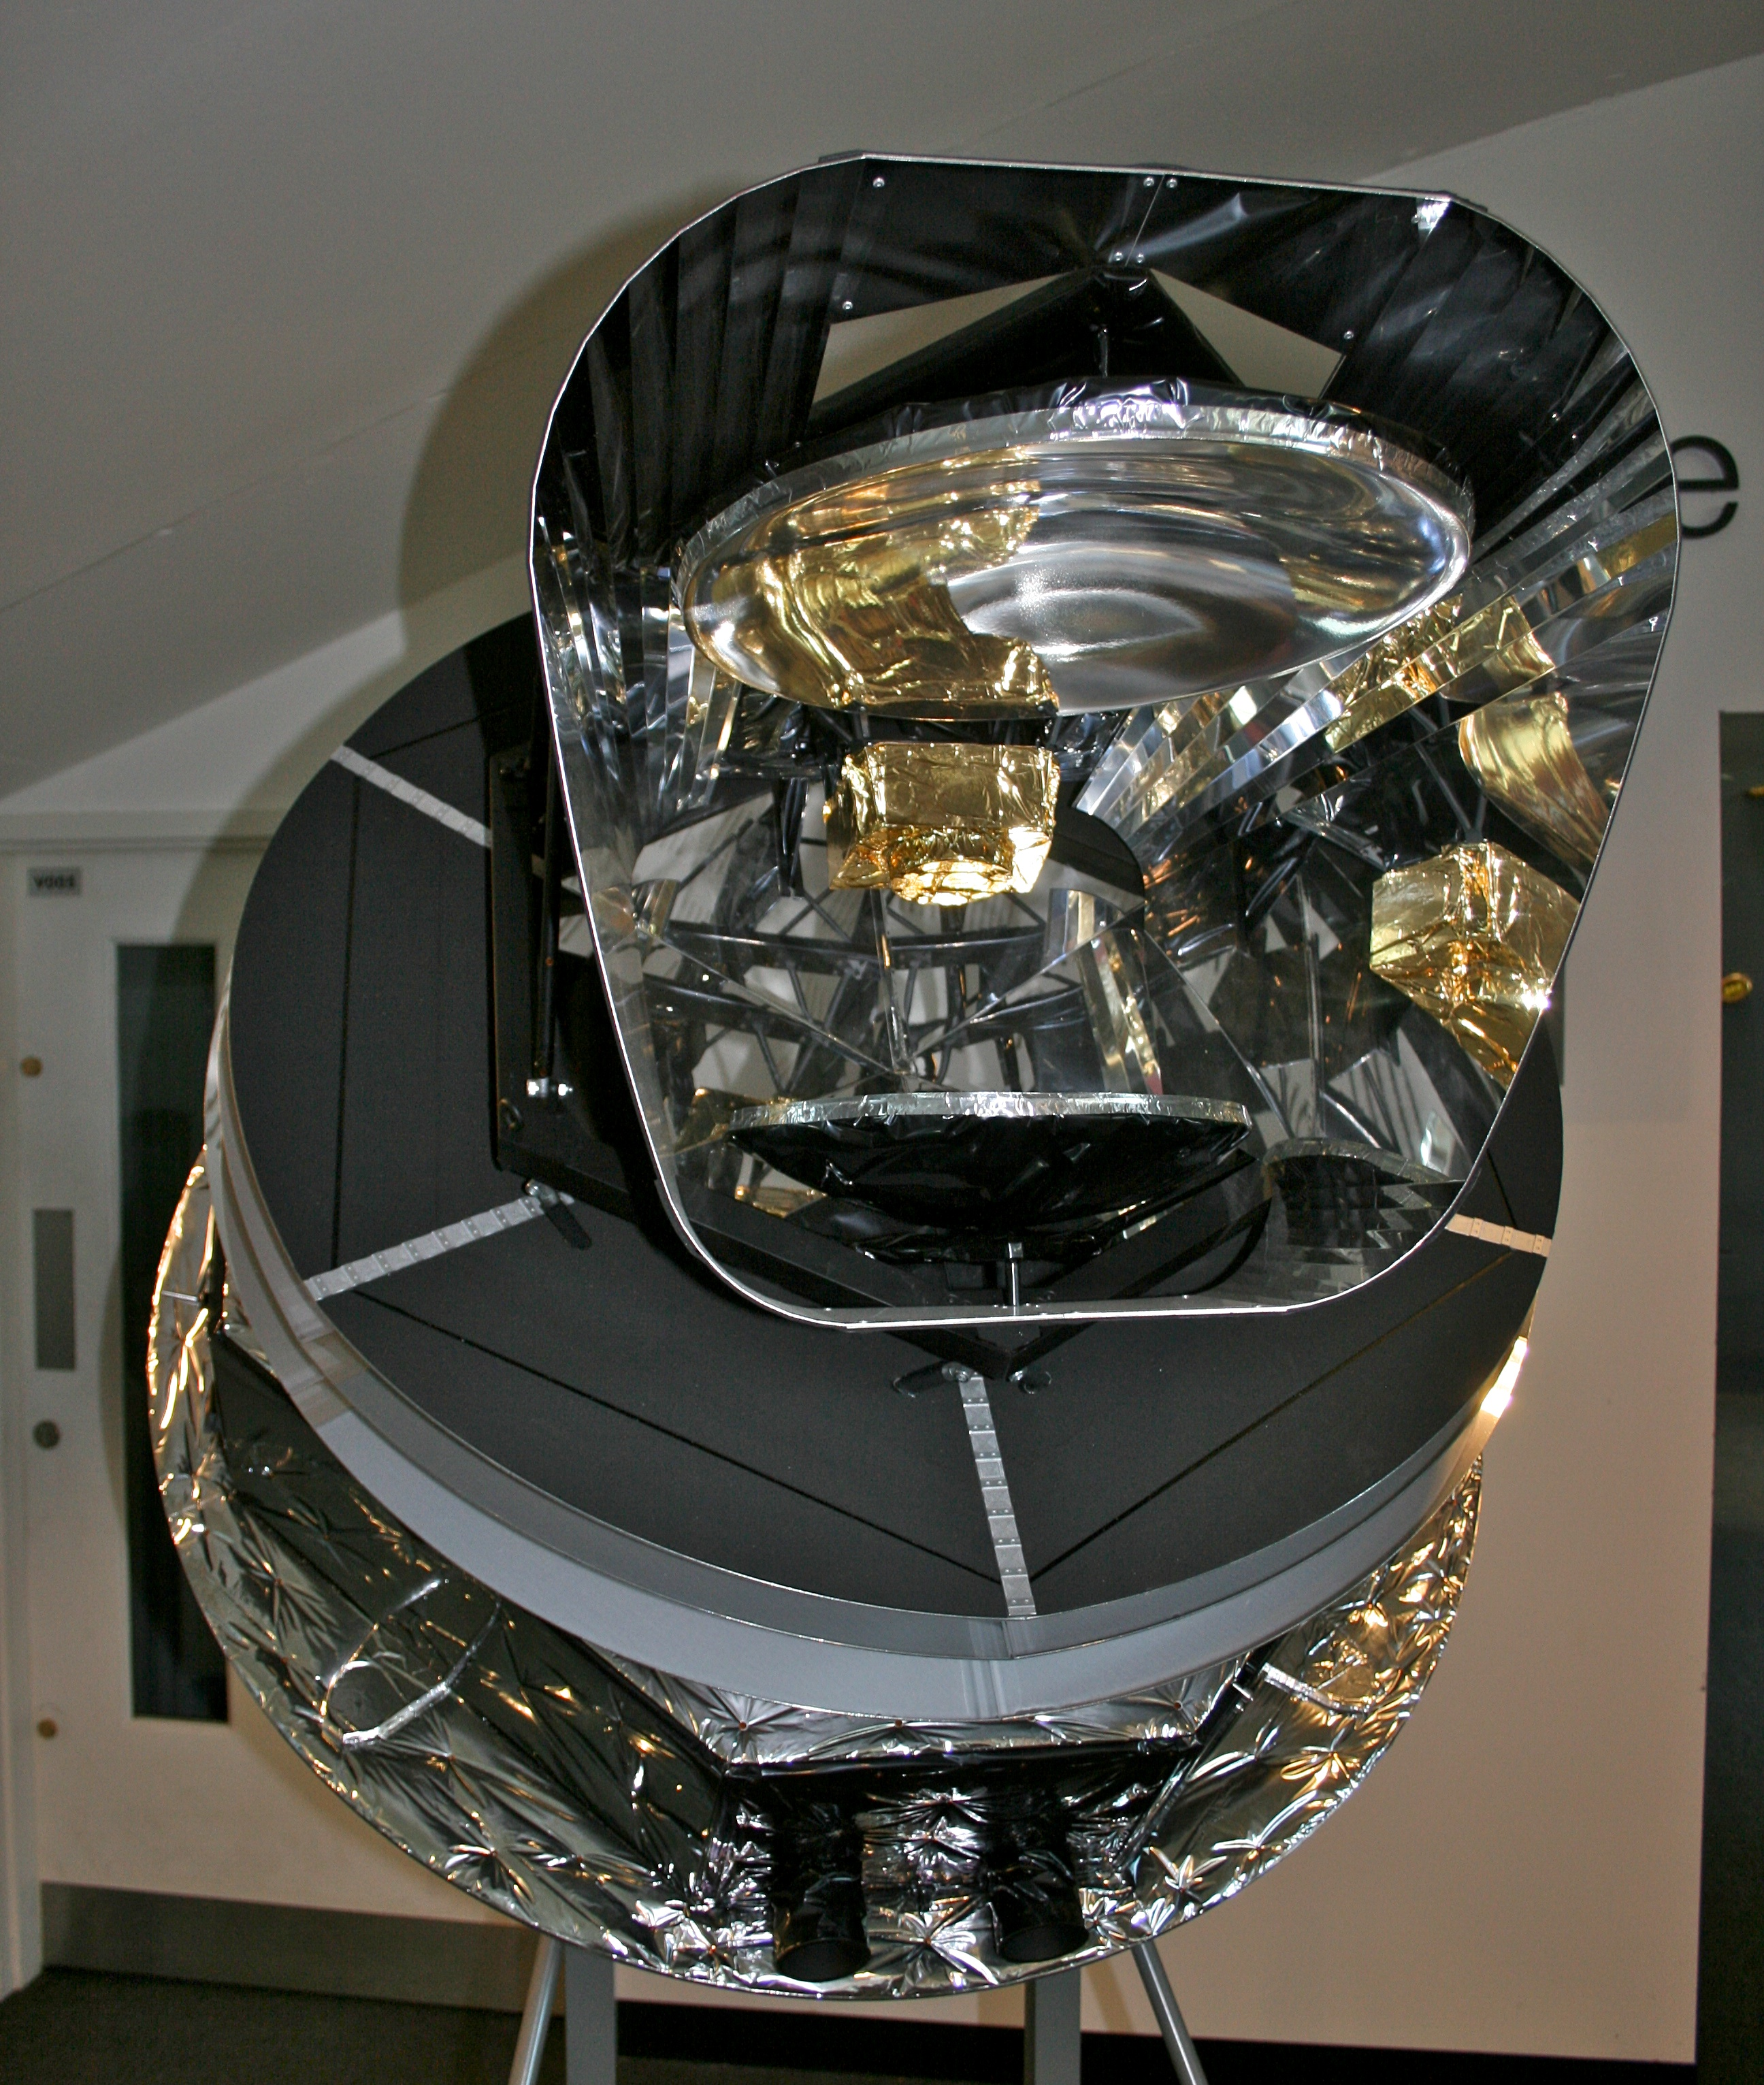
\includegraphics[width=0.45\textwidth]{Model_of_the_Planck_Satellite_1.jpg}};
		\end{tikzpicture}		
	\end{center}
\end{frame}
	
\begin{frame}{Planck}
	\begin{center}
		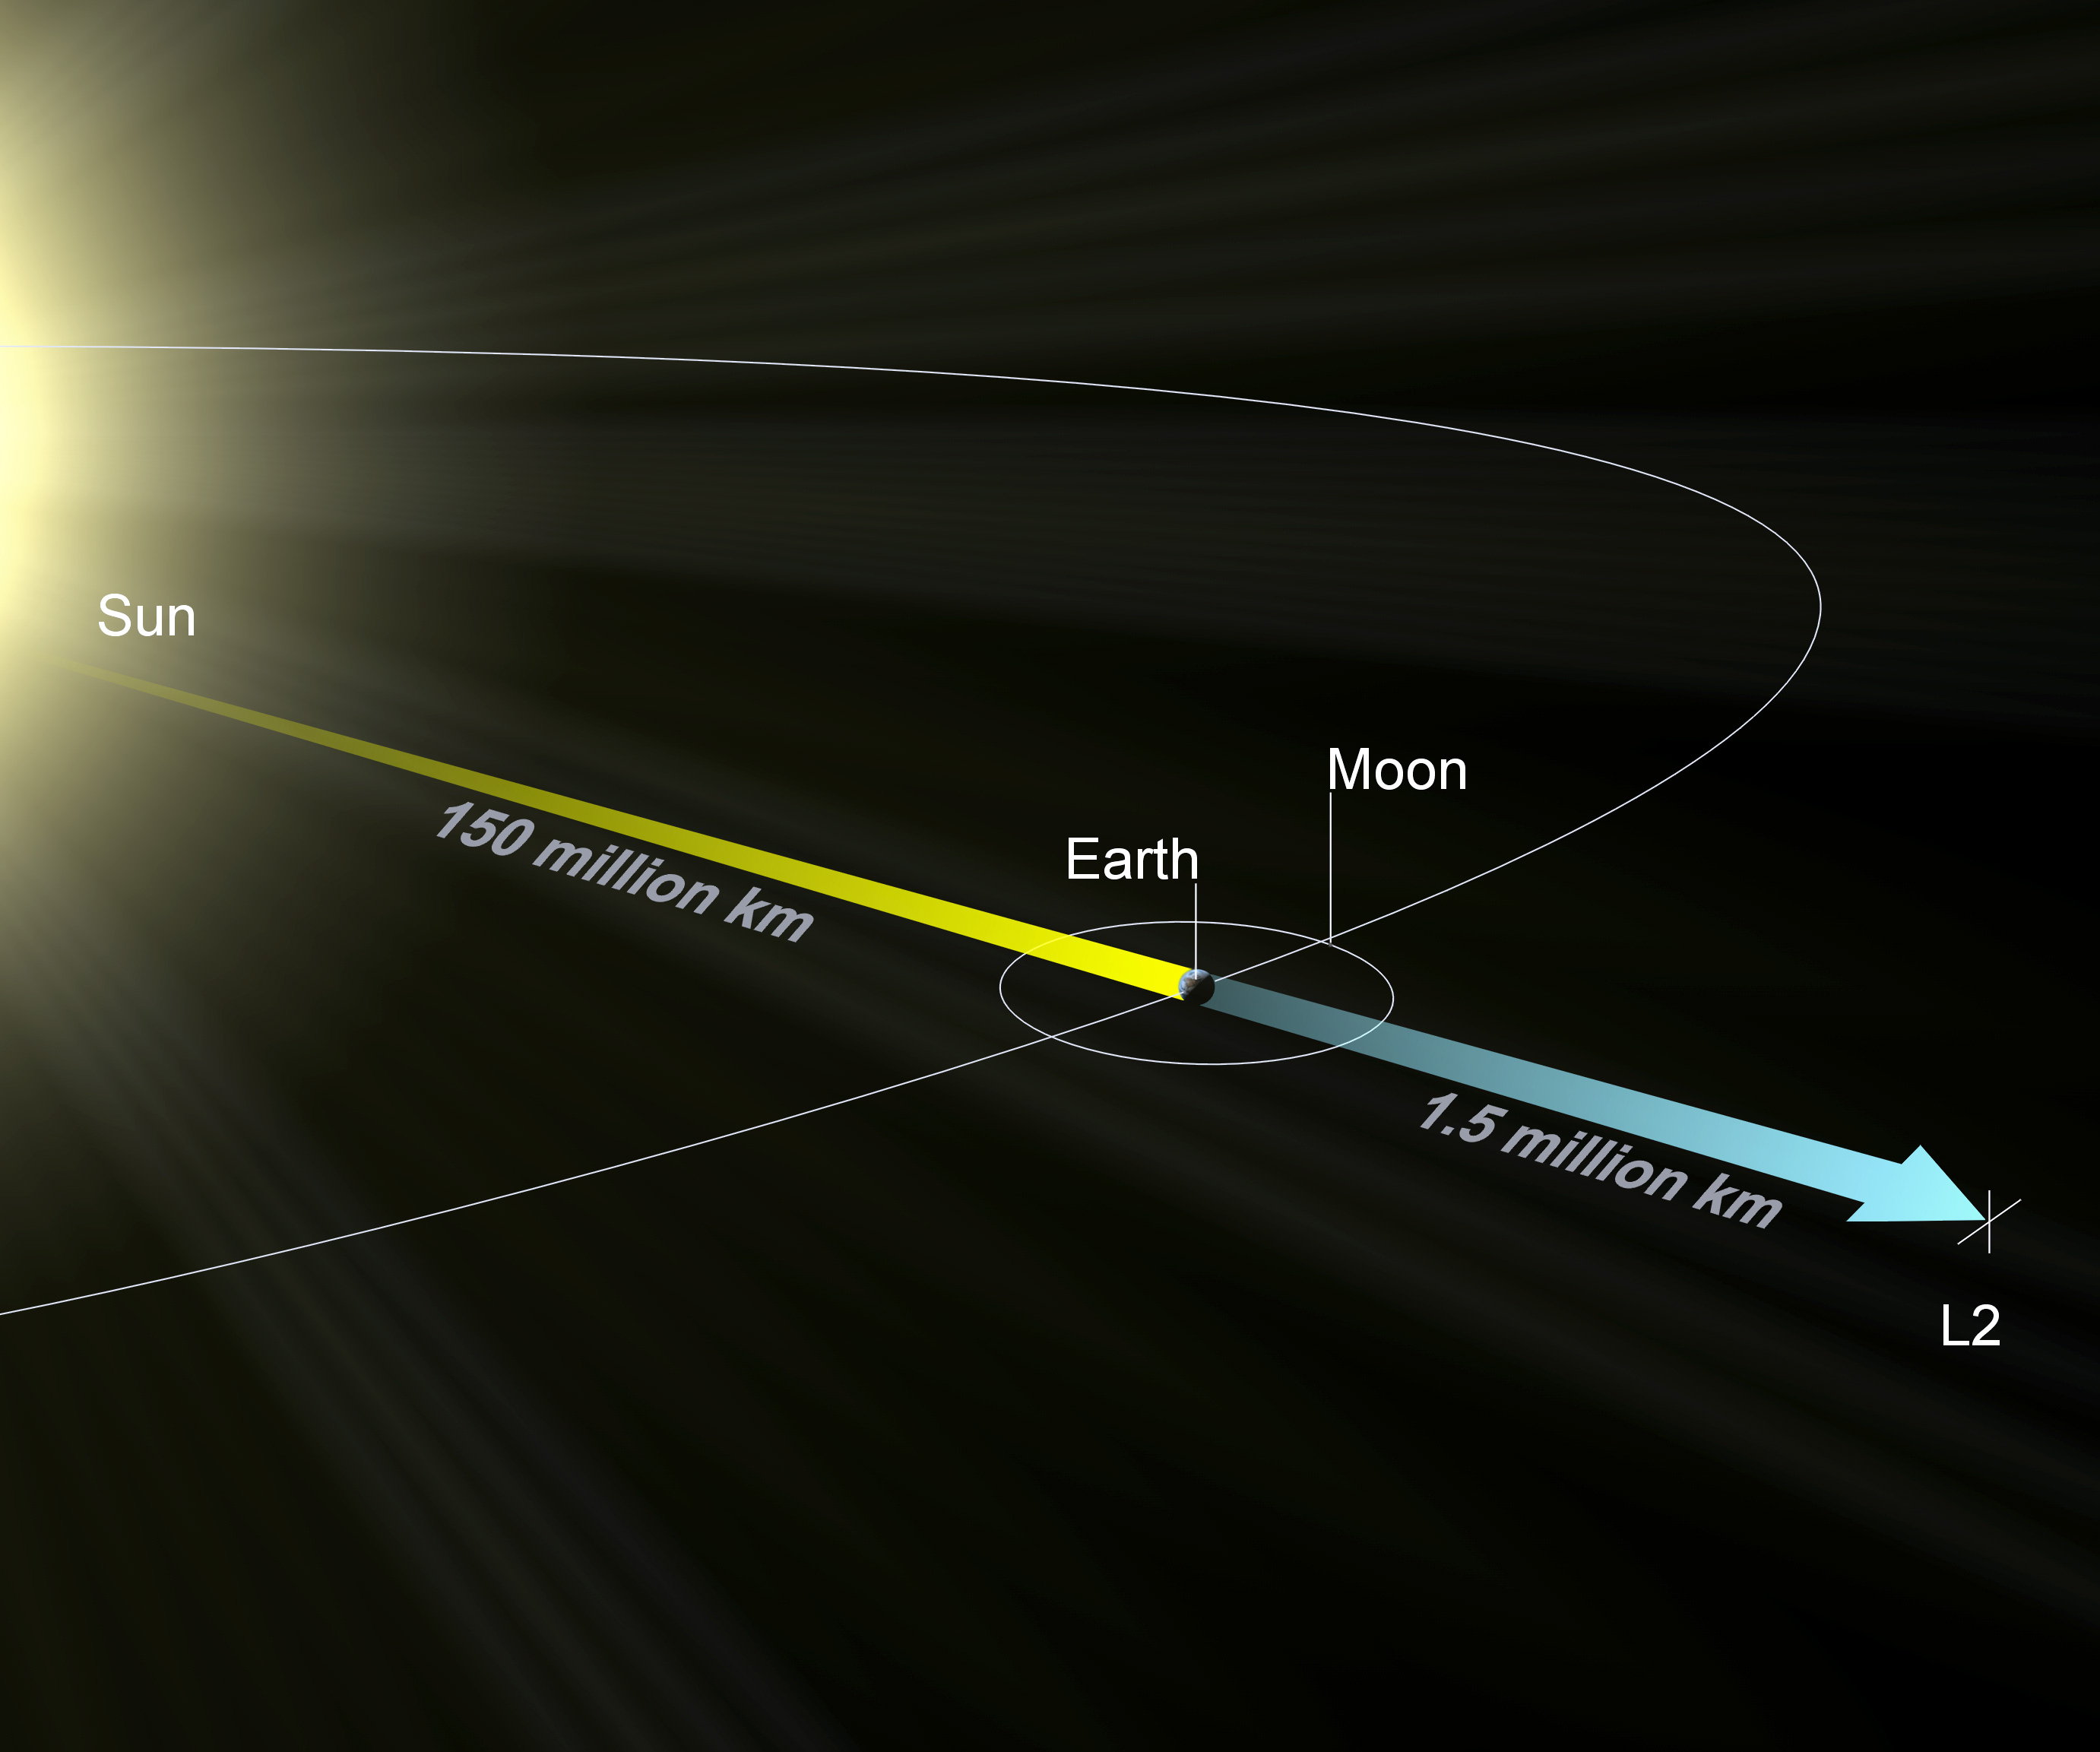
\includegraphics[width=0.8\textwidth]{L2_rendering.jpg}		
	\end{center}
\end{frame}

\begin{frame}{Weltraumteleskope}
	\begin{center}
	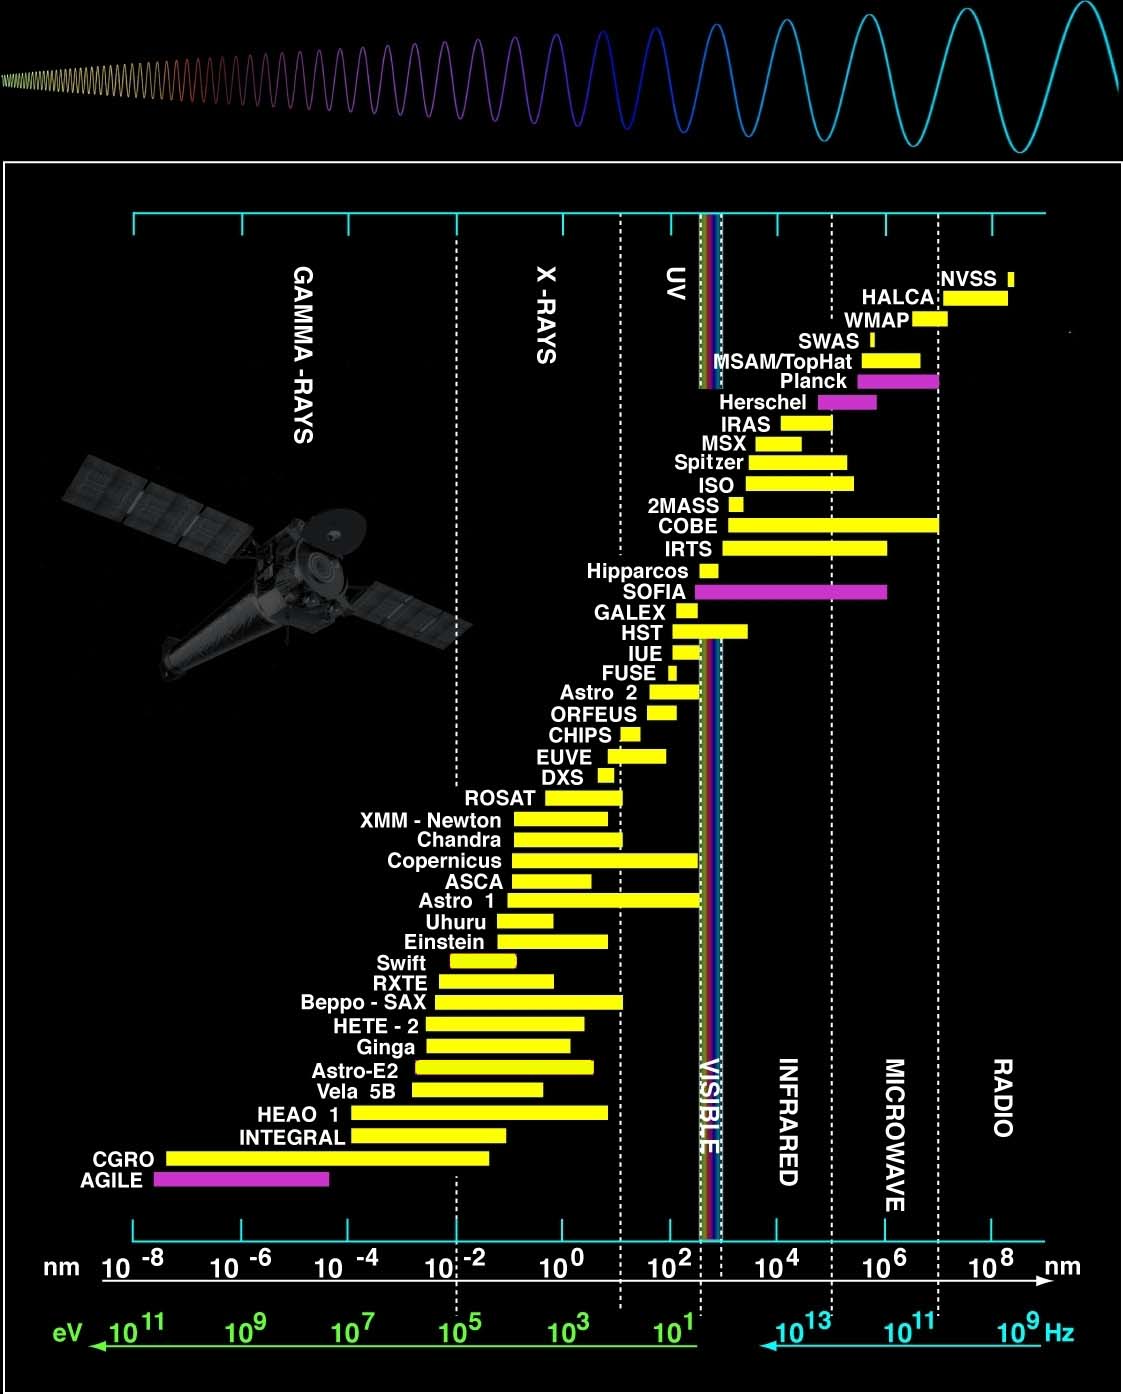
\includegraphics[height=0.8\textheight]{Space_telescopes.png}		
	\end{center}
\end{frame}

\begin{frame}
	\frametitle{Kosmologische Rotverschiebung}
	
	\begin{center}
		\begin{tikzpicture}
		\node at (0,0) {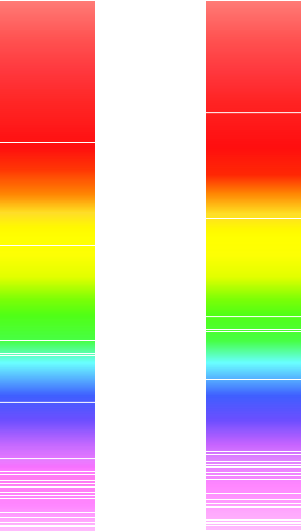
\includegraphics[height=0.7\textheight]{rotverschiebung.png}};
		\node[rotate=-90] at (2.3,0) {Die meisten Galaxien};
		\node at (0,-4) {$H_0 = (67.74 \pm 0.46) \mathrm{\frac{km}{s \cdot Mpc}}$};
		\node[rotate=90] at (-2.3,0) {Unsere Sonne};
		\node at (-5,-1.6) {
\includegraphics[width=0.3\textwidth]{prisma.png}};
		\node at (-5,1.6) {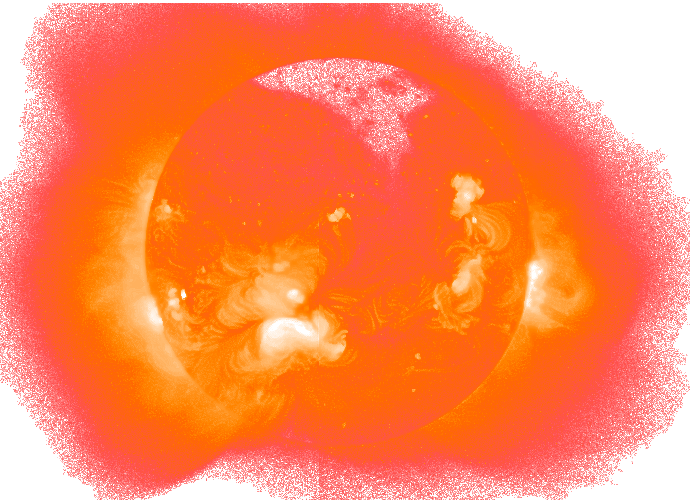
\includegraphics[width=0.3\textwidth]{Sun_in_X-Ray.png}};
		\end{tikzpicture}		
	\end{center}
	
\end{frame}

\begin{frame}
	\frametitle{Hintergrundstrahlung}
	\begin{center}
		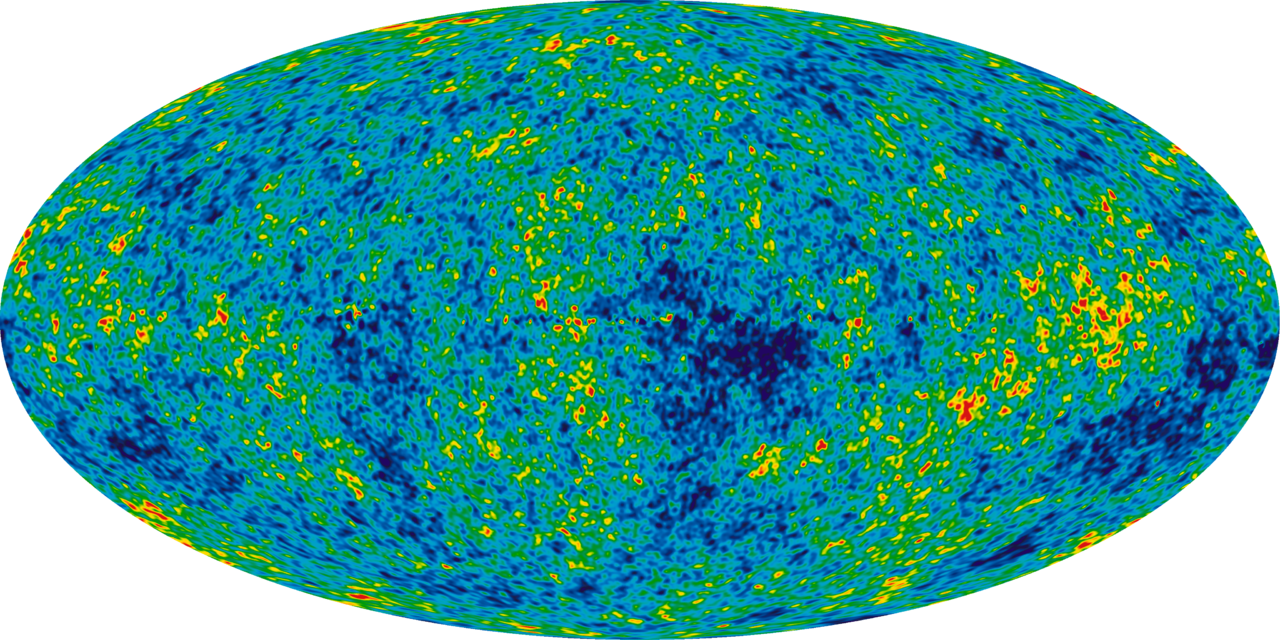
\includegraphics[width=\textwidth]{hintergrundstrahlung.png}
	\end{center}
\end{frame}
	
\begin{frame}
	\frametitle{Expansion des Universums}
	\begin{center}
		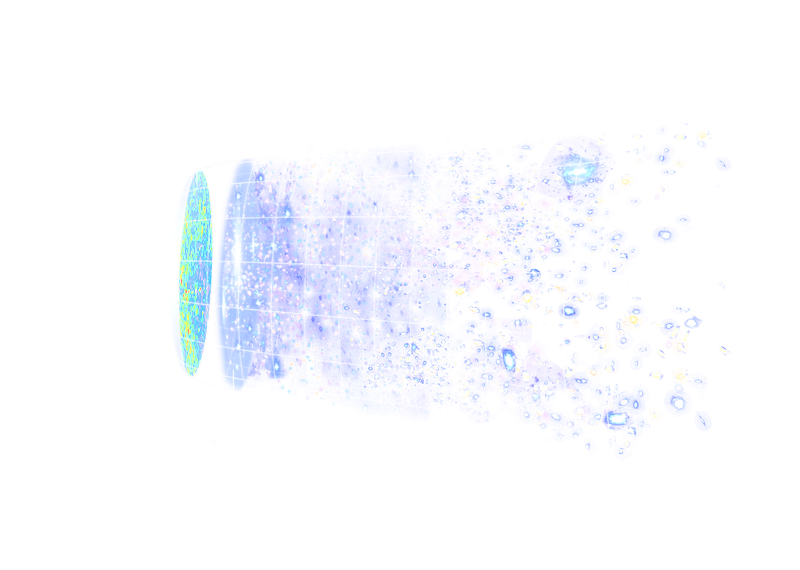
\includegraphics[width=\textwidth]{expansion.png}
	\end{center}
\end{frame}
	
\begin{frame}
	\centering
	\huge{Dunkle Materie}
\end{frame}

\begin{frame}
	\frametitle{Rotationsgeschwindigkeit von Galaxien}
	\begin{center}
		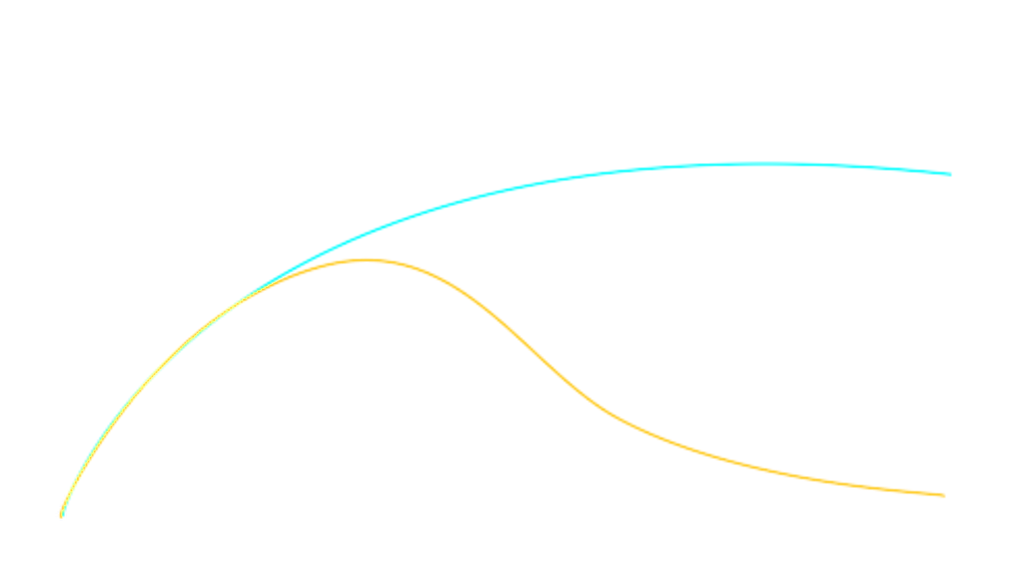
\includegraphics[height=0.4\textheight]{dark_matter.png}
		
		
		\movie[autostart,loop,width=0.8\textwidth,height=0.4\textheight]{Rotationskurven}{rotationskurven.webm}
	\end{center}
\end{frame}

\begin{frame}
	\frametitle{Einstein-Ringe -- Microlensing}
	\begin{center}
				\vspace*{-1em}
		\hspace*{-2em}
			\begin{tikzpicture}
			\node at (-2,-3.5) {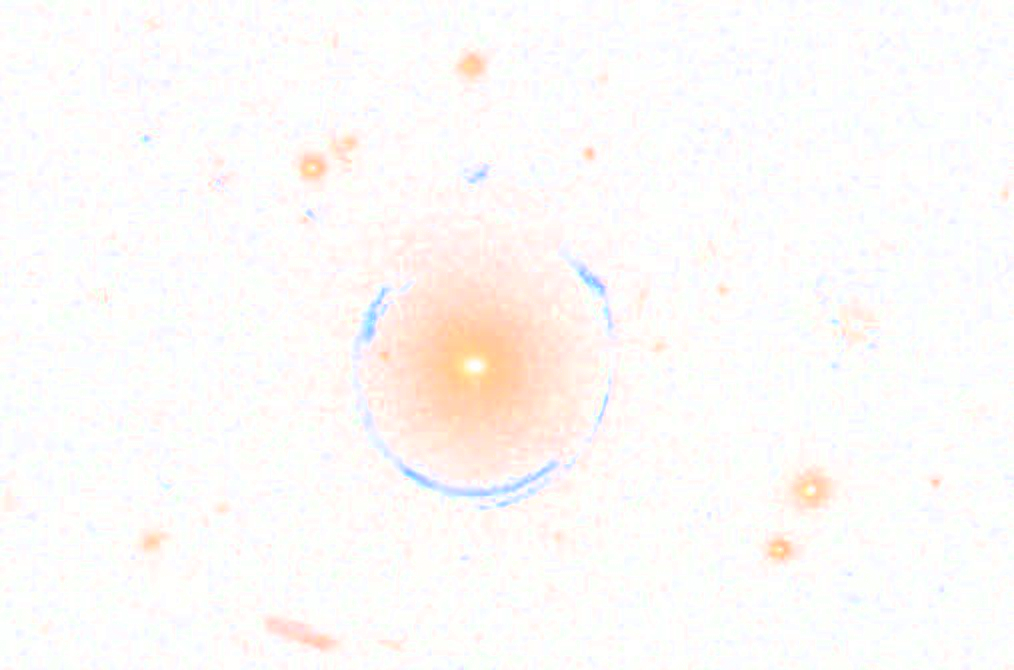
\includegraphics[height=0.5\textheight]{microlensing.png}};
			\node at (4,-3.5) {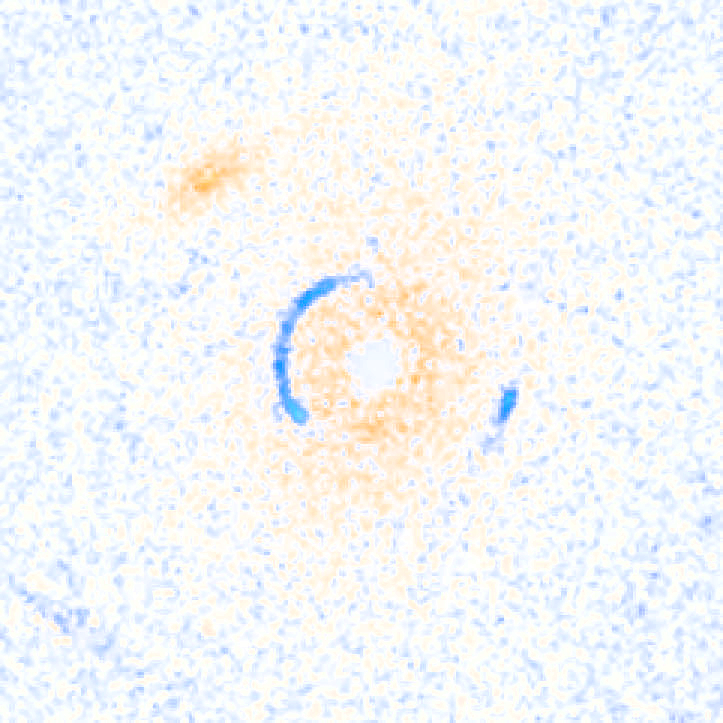
\includegraphics[height=0.5\textheight]{microlensing2.png}};
			\node at (0,0) {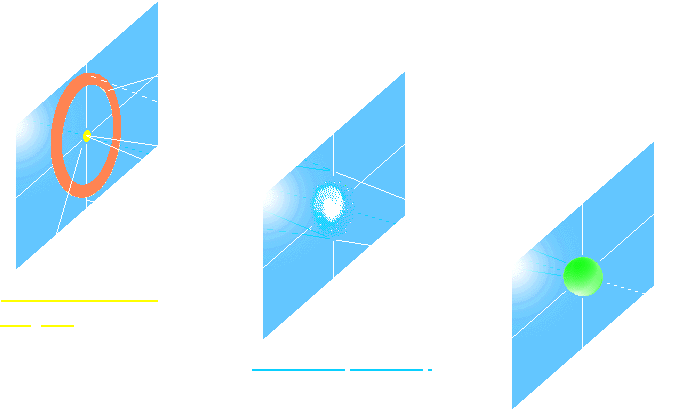
\includegraphics[height=0.5\textheight]{Einstein-Ring-schem_de.png}};
			\end{tikzpicture}		
	\end{center}
\end{frame}

\begin{frame}
	\centering
	\huge{Dunkle Energie}
\end{frame}

\begin{frame}{Supernova 1a -- Standardkerzen}
	\centering
	\begin{tikzpicture}
	\node at (0,0) {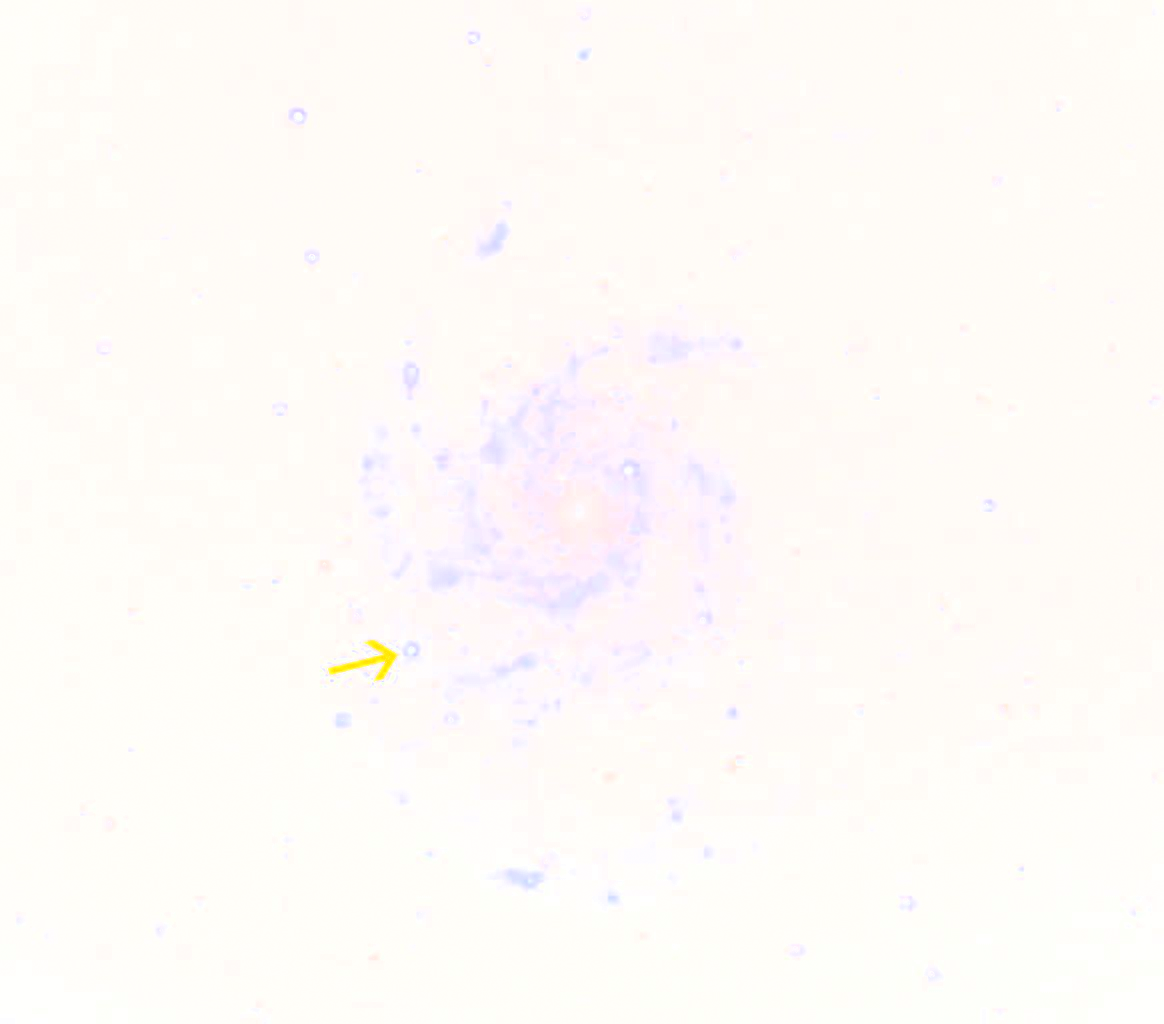
\includegraphics[width=0.8\textwidth]{supernova.png}};
	\end{tikzpicture}	
	
\end{frame}

\begin{frame}{Dunkle Materie \& Dunkle Energie}
	\centering
	\hspace*{-1em}
	\begin{tikzpicture}
	\node at (0,0) {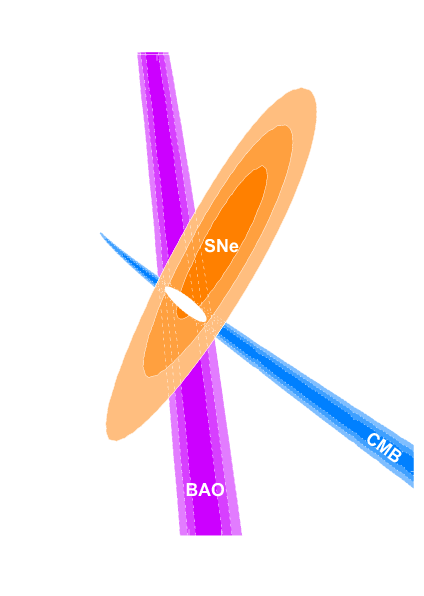
\includegraphics[height=0.8\textheight]{DEkosowski.png}};
	\node at (6,0) {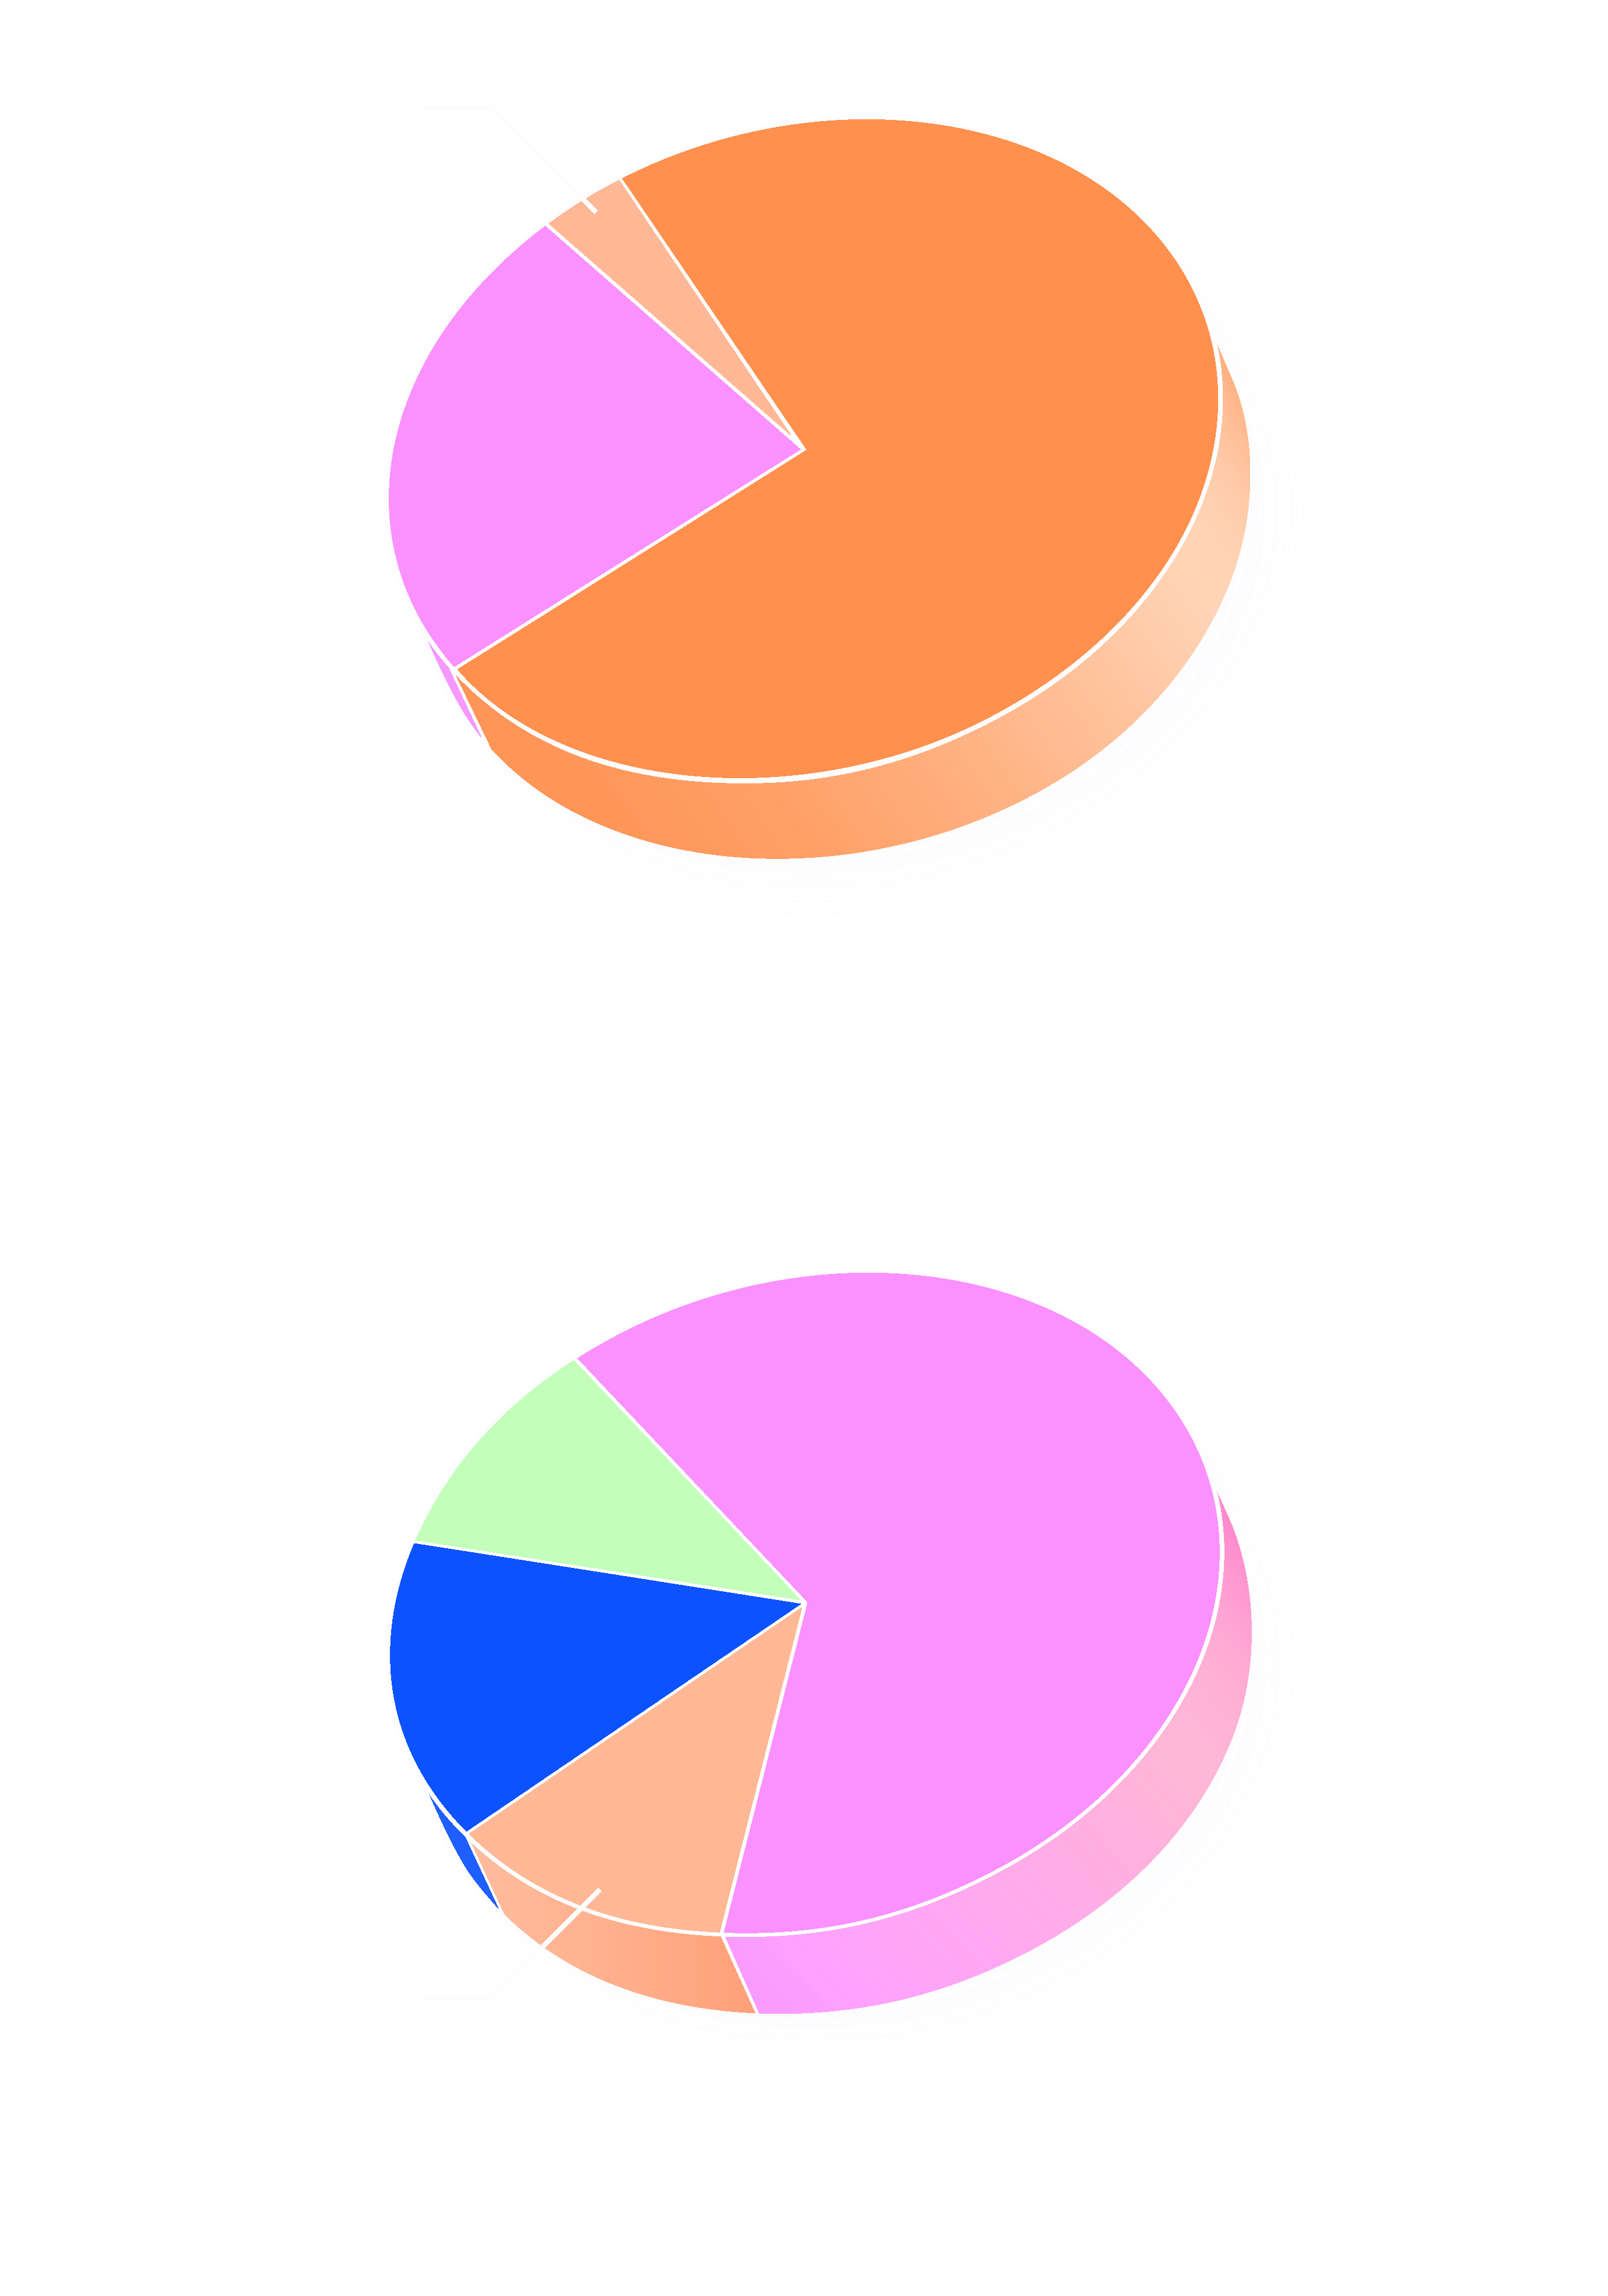
\includegraphics[height=0.8\textheight]{WMAP_2008_universe_content_de.png}};
	\end{tikzpicture}	
	 
\end{frame}

\begin{frame}
	\centering
	\huge{Gravitationswellen}
\end{frame}

\begin{frame}
	\frametitle{Allgemeine Relativitätstheorie}
	
	\begin{tikzpicture}[scale=6]
	\node[] at (-1.0,0) {\huge $R_{\mu\nu} - (\frac{R}{2} - \Lambda) g_{\mu\nu} =\frac{8 \pi G}{c^4} T_{\mu\nu}$};
	\end{tikzpicture}
\end{frame}

\begin{frame}
	\frametitle{LIGO}
	\begin{center}
		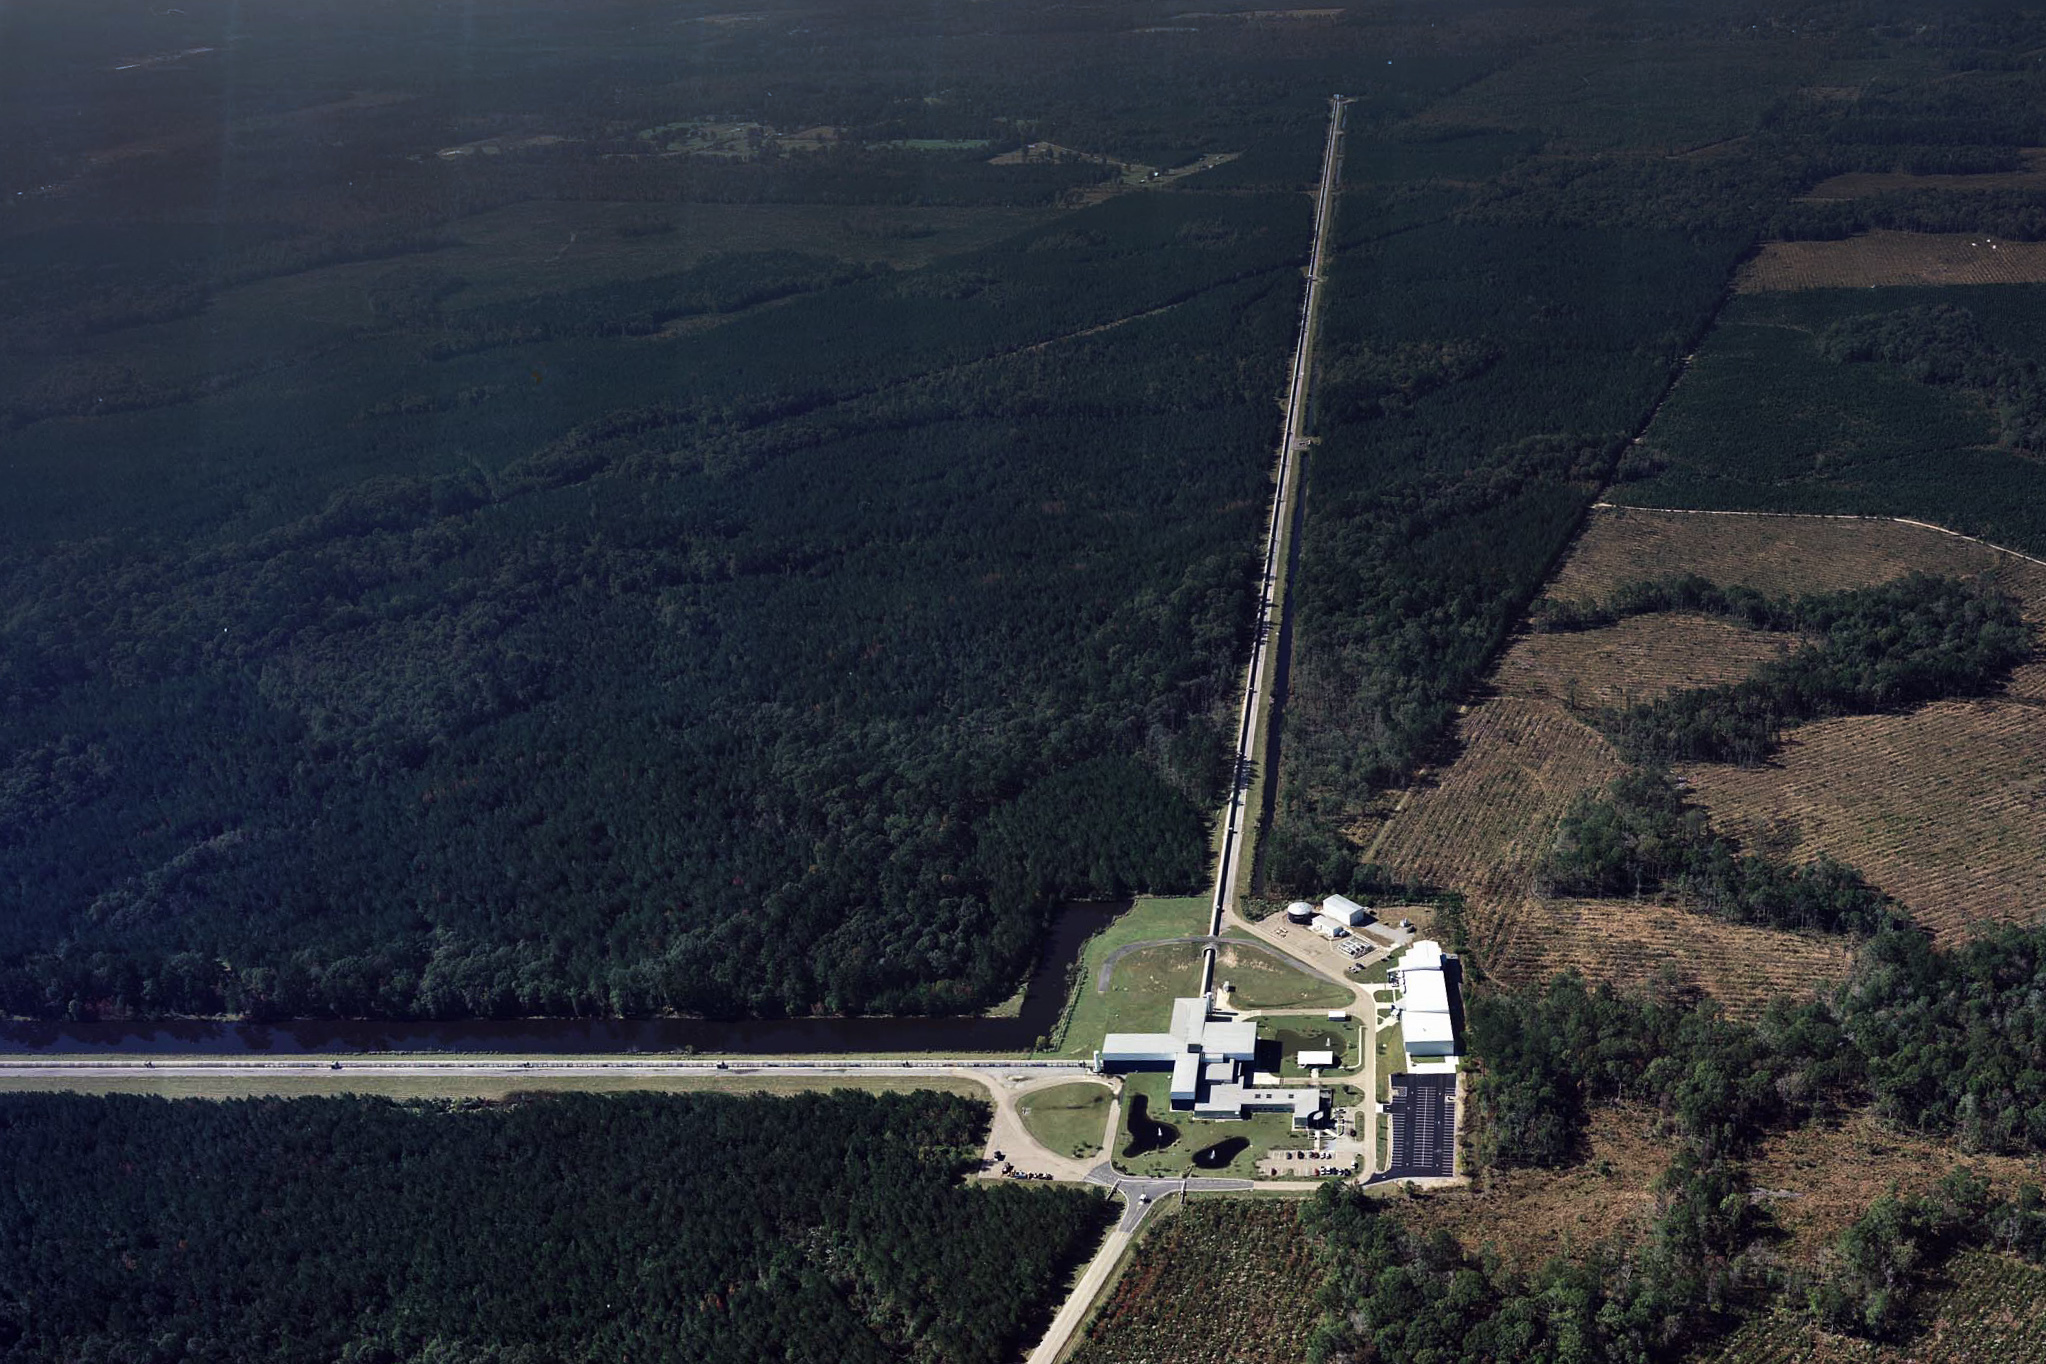
\includegraphics[width=\textwidth]{aerial_ligo5_300.jpg}
	\end{center}
\end{frame}

\begin{frame}
	\frametitle{Messprinzip}
	\begin{center}
		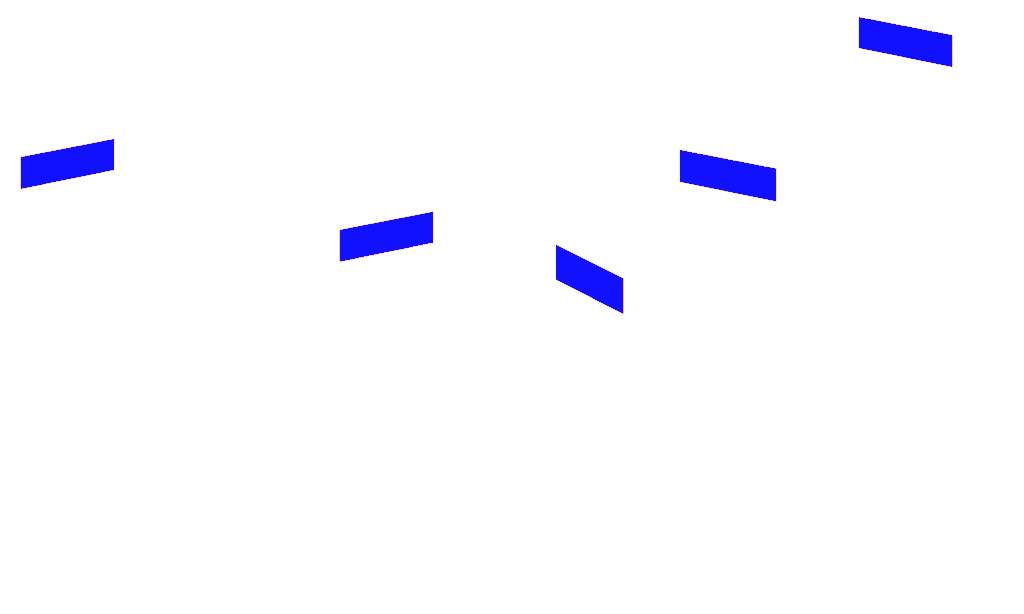
\includegraphics[width=\textwidth]{ligo.png}
	\end{center}
\end{frame}

\begin{frame}
	\frametitle{Gravitationswellen}
	\begin{center}
		\movie[autostart,width=0.8\textwidth,height=0.5\textheight]{Gravitationswellen}{chirp.webm}
	\end{center}
\end{frame}

\usebackgroundtemplate{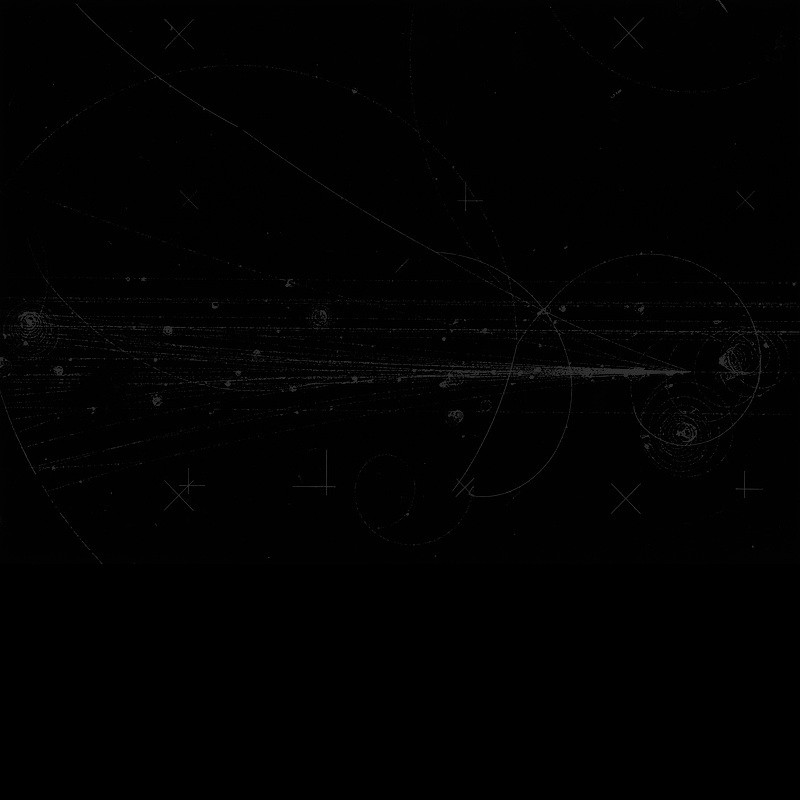
\includegraphics[width=\paperwidth]{bubble.jpg}}%
\begin{frame}
	\centering
	\huge{Powers of Ten -- Teil II}
\end{frame}

\begin{frame}
	\centering
	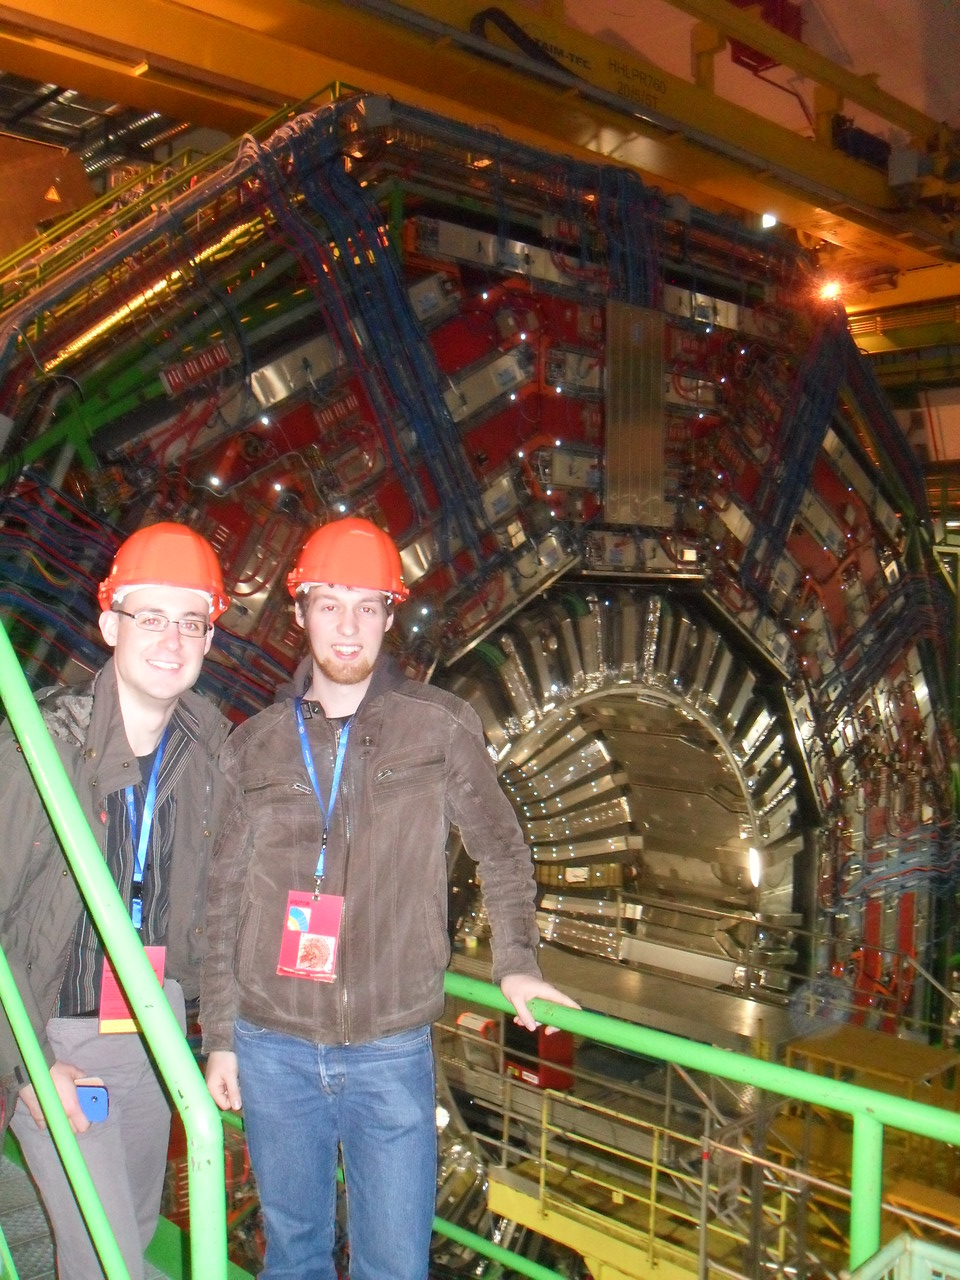
\includegraphics[height=0.8\textheight]{SDC13090.JPG}
\end{frame}

\begin{frame}
	\centering
	\huge{Das Higgs-Boson}
\end{frame}

\begin{frame}{Der Large Hadron Collider}
	\centering
	\begin{tikzpicture}
	\node at (0,0) {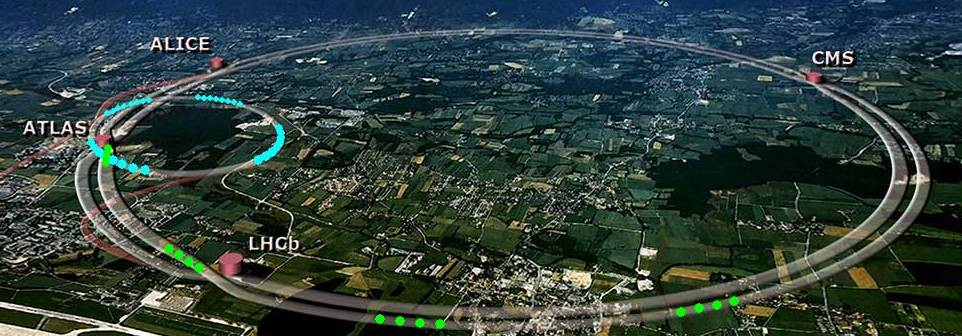
\includegraphics[width=\textwidth]{lhc-aerial.jpg}};
	\node at (3,-4) {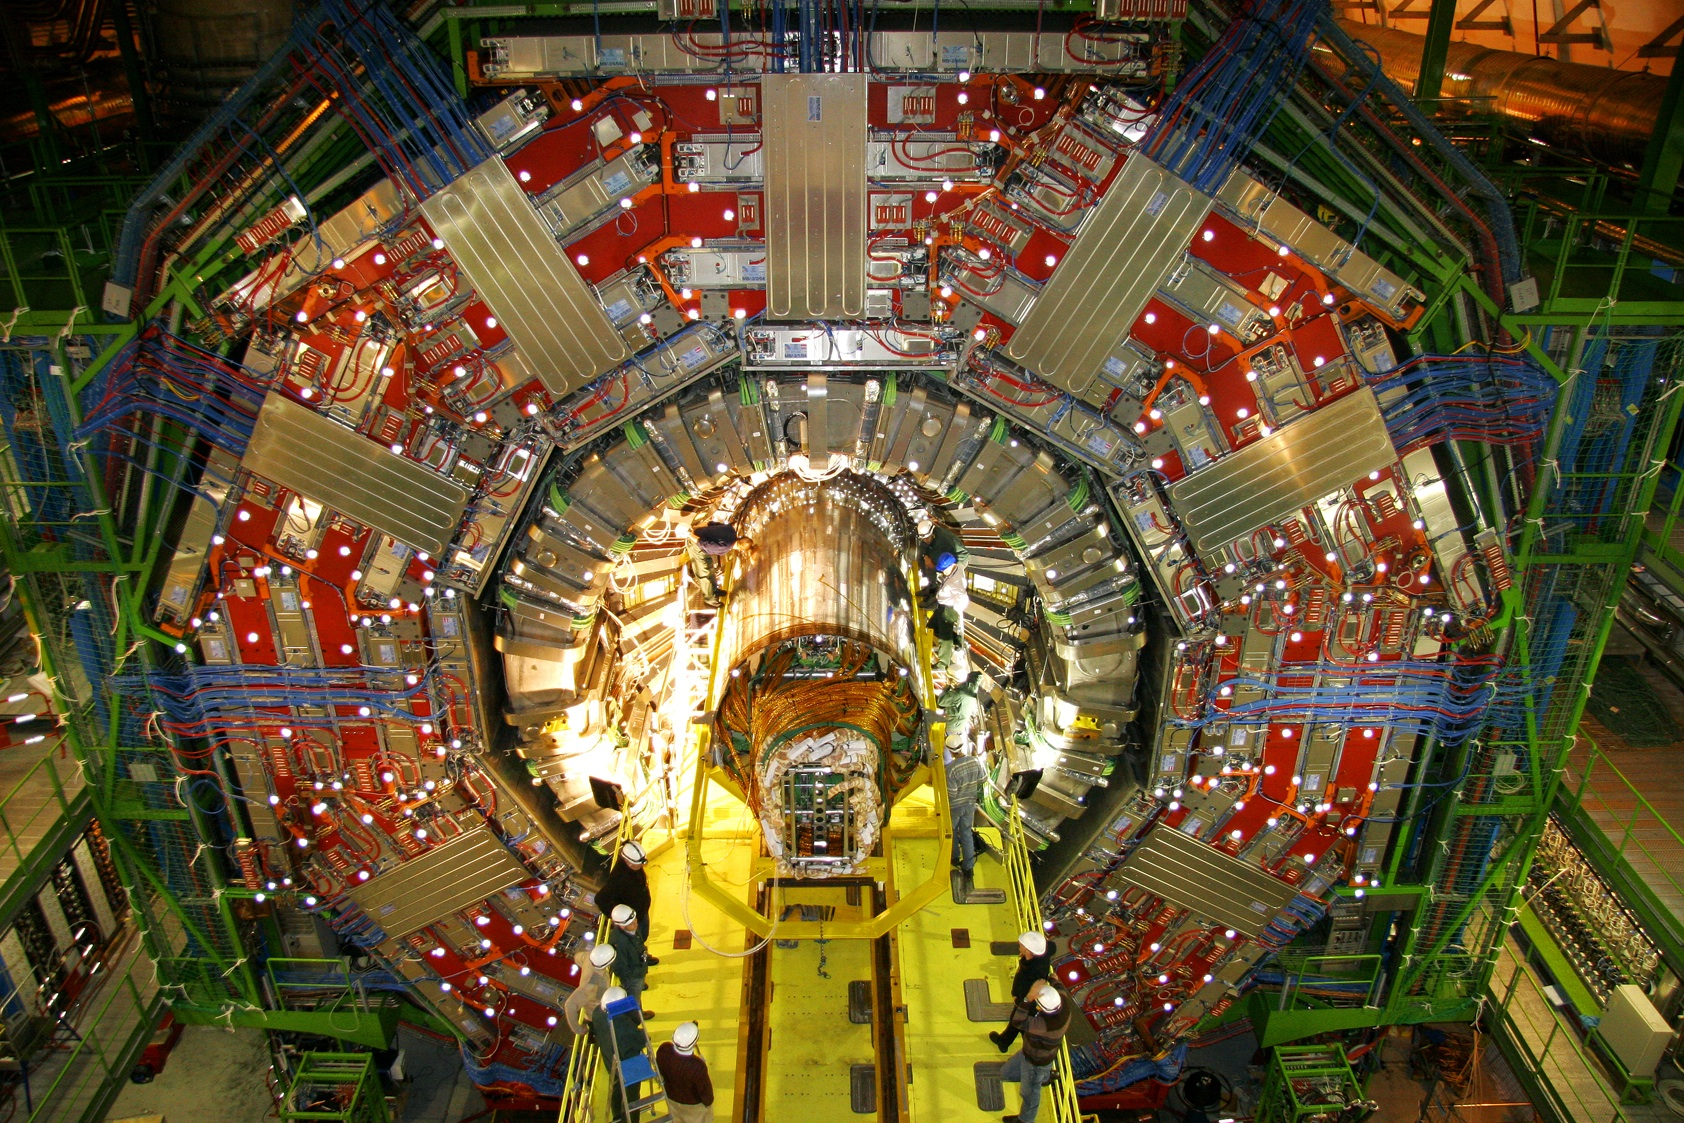
\includegraphics[height=0.3\textheight]{bul-pho-2007-079.jpg}};
    \node at (-3,-4) {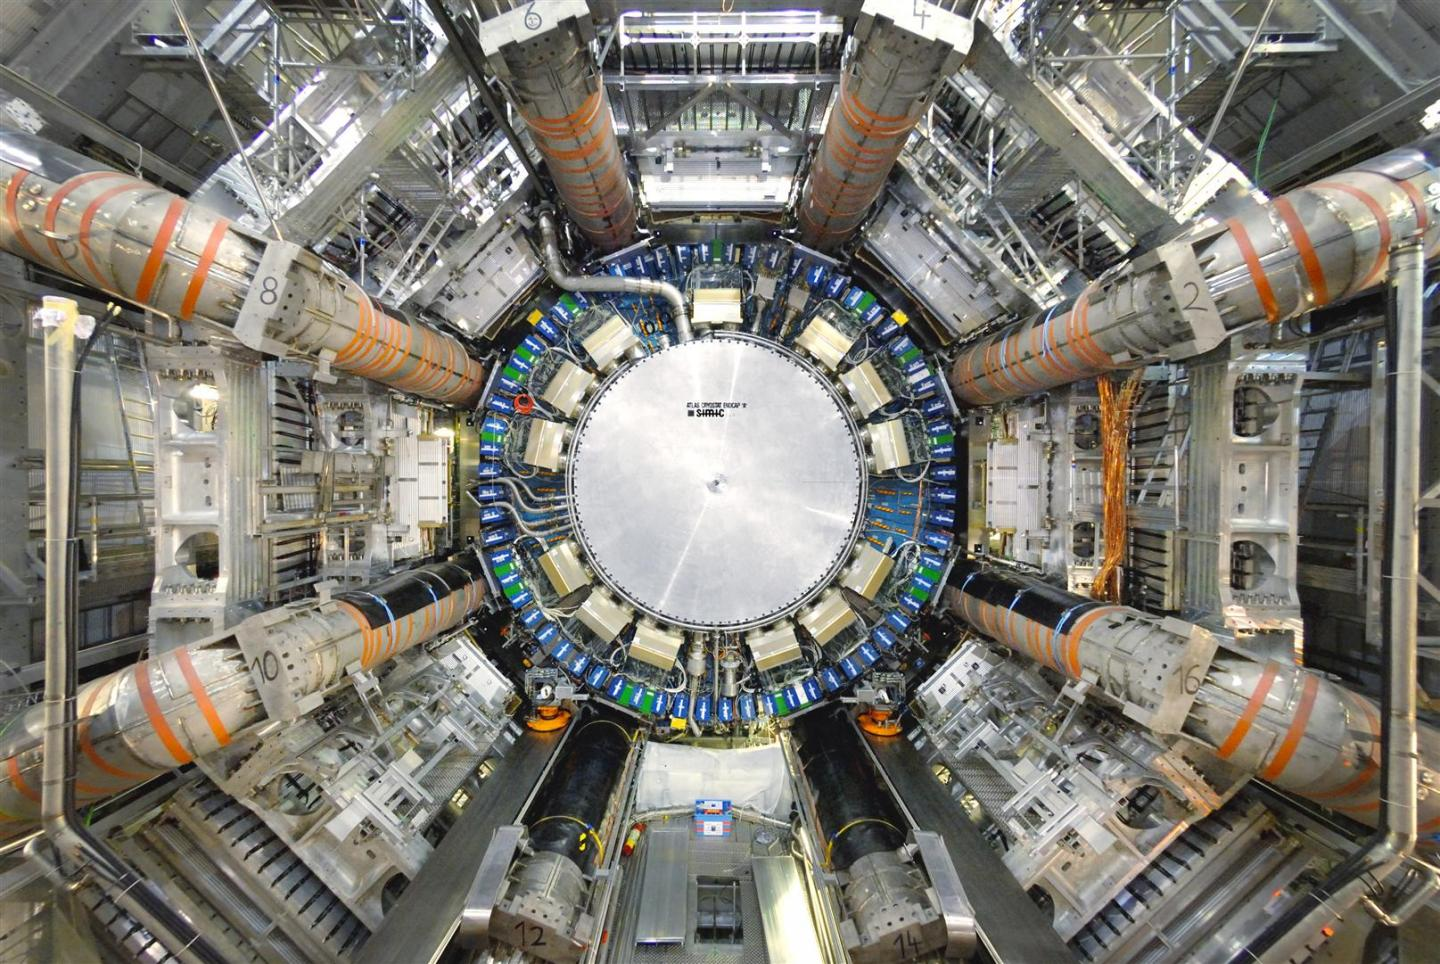
\includegraphics[height=0.3\textheight]{atlas.jpeg}};
	\end{tikzpicture}
	
\end{frame}

\begin{frame}
	\centering
	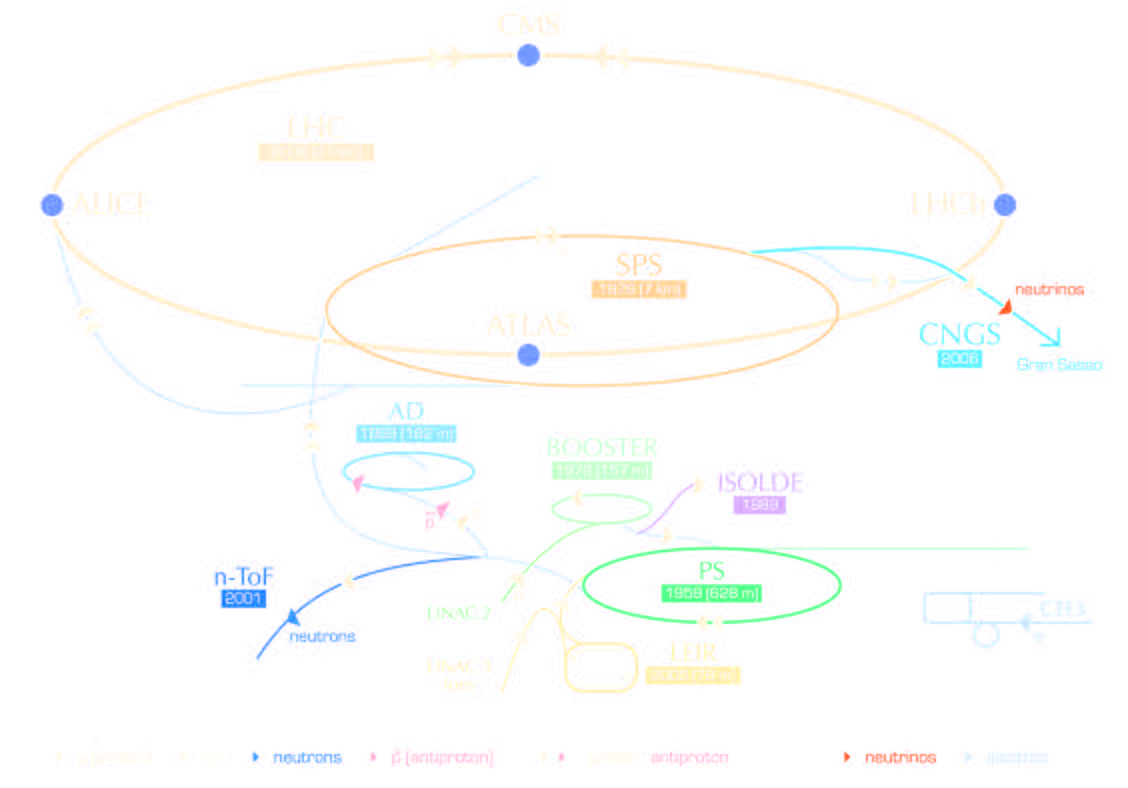
\includegraphics[width=\textwidth]{cern.png}
\end{frame}

\begin{frame}
	\frametitle{Der CMS Detektor}
	\begin{center}
		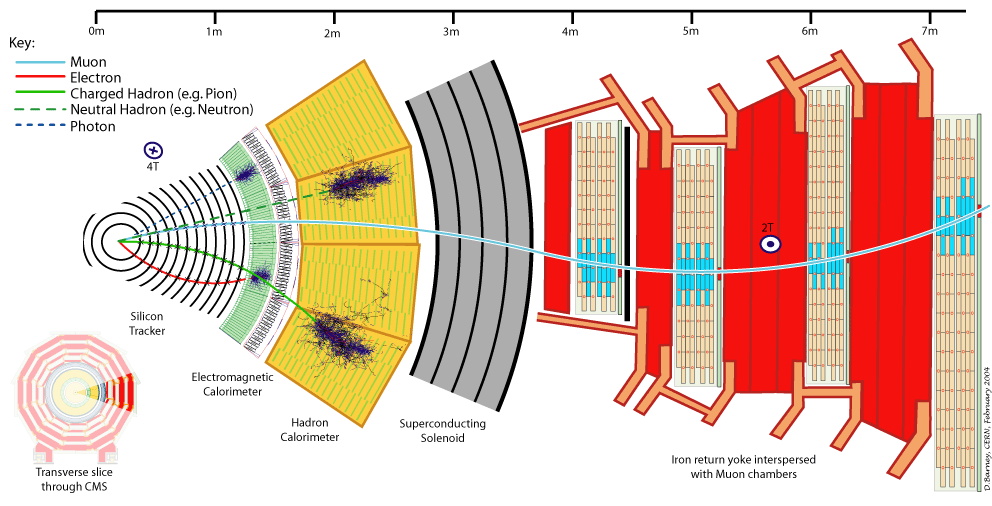
\includegraphics[width=\textwidth]{messprinzip.png}
	\end{center}
\end{frame}

\begin{frame}
	\frametitle{Ein echtes Ereignis}
	\begin{center}
		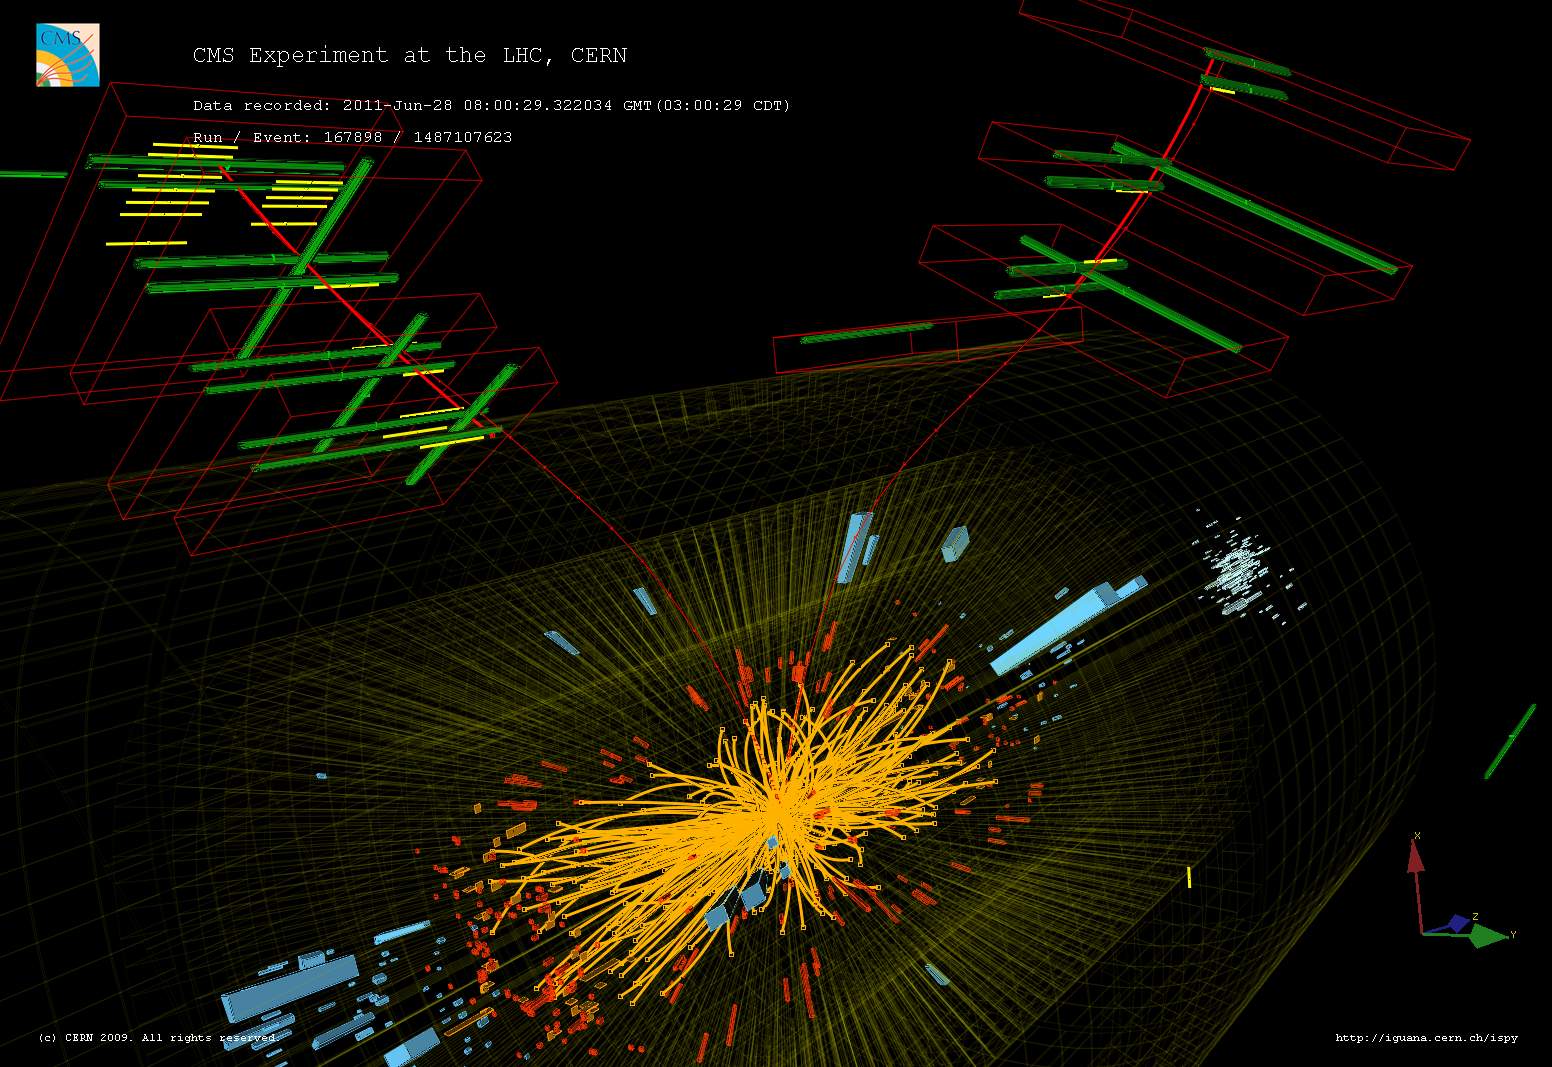
\includegraphics[width=\textwidth]{dimuon_event.png}
	\end{center}
\end{frame}

\begin{frame}
	\frametitle{Die Entdeckung des Higgs Bosons}
	\begin{center}
		\movie[autostart,width=\textwidth,height=0.7\textheight]{\vspace{4em}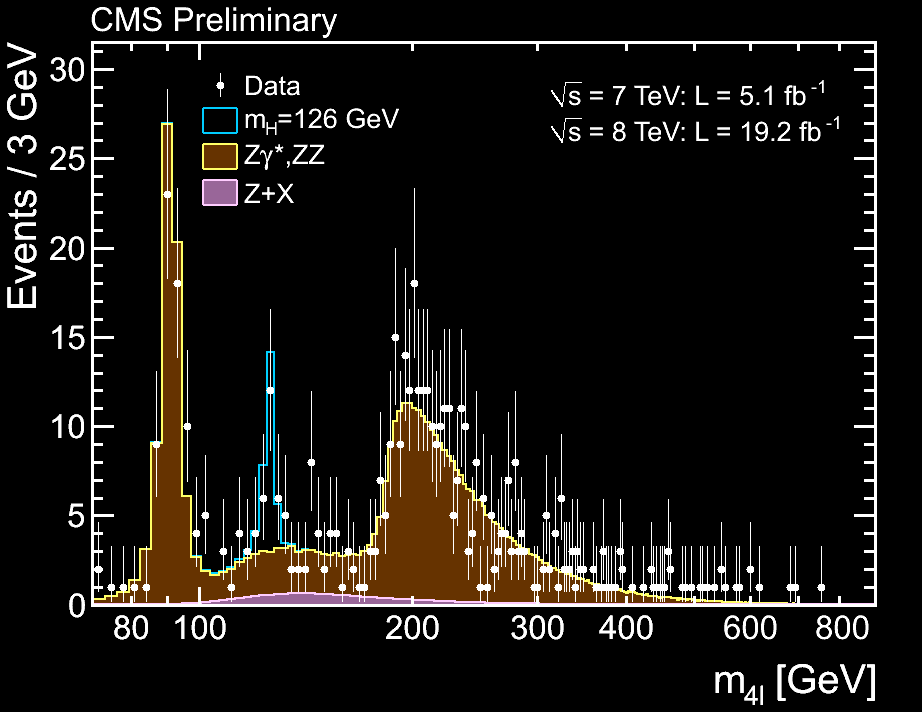
\includegraphics[width=0.8\textwidth]{higgs_last_frame.png}}{higgs.webm}
	\end{center}
\end{frame}

\begin{frame}
	\centering
	\huge{Das Standardmodell der Teilchenphysik}
\end{frame}

\begin{frame}
	\frametitle{Höchste Energien: LHC \& CMS}
	\begin{center}
		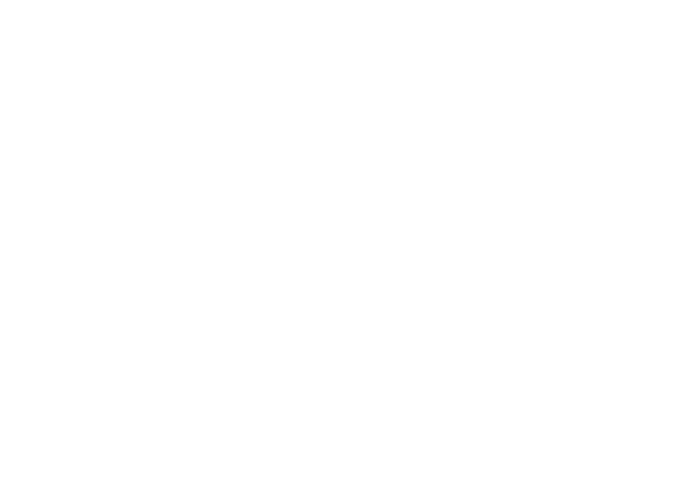
\includegraphics[width=\textwidth]{dimuon.png}
	\end{center}
\end{frame}

\begin{frame}
	\frametitle{Höchste Luminosität: KEKB \& Belle}
	\begin{center}
		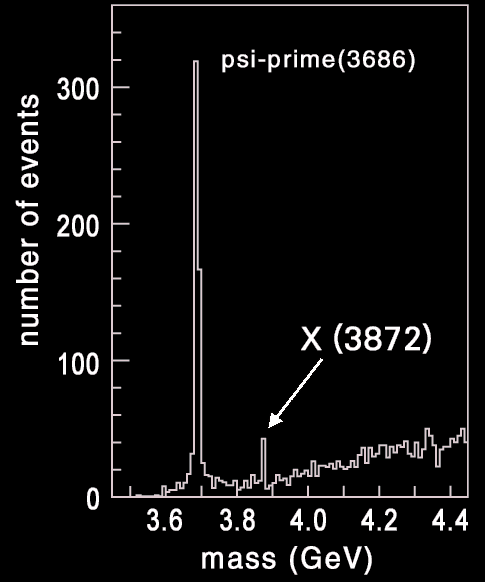
\includegraphics[width=0.6\textwidth]{belle.png}
	\end{center}
\end{frame}

\begin{frame}
	\frametitle{Das Standardmodell der Teilchenphysik}
		\begin{align*}
		\mathcal{L} &= -\frac{1}{4} F_{\mu\nu} F^{\mu\nu} & & \textrm{Fundamentale Kräfte}\\
		&+ i \bar{\psi} \slashed{D} \psi + \mathrm{h.c.} & & \textrm{Wechselwirkung mit Materie}\\
		&+ \psi_i y_{ij} \psi_j \phi + \mathrm{h.c.} & & \textrm{Masse und CP Verletzung}\\
		&+ |D_\mu \phi|^2 - V(\phi) \quad  & & \textrm{Higgs Sektor}
		\end{align*}
\end{frame}

\begin{frame}
	\frametitle{Das Standardmodell der Teilchenphysik}
	\begin{center}
		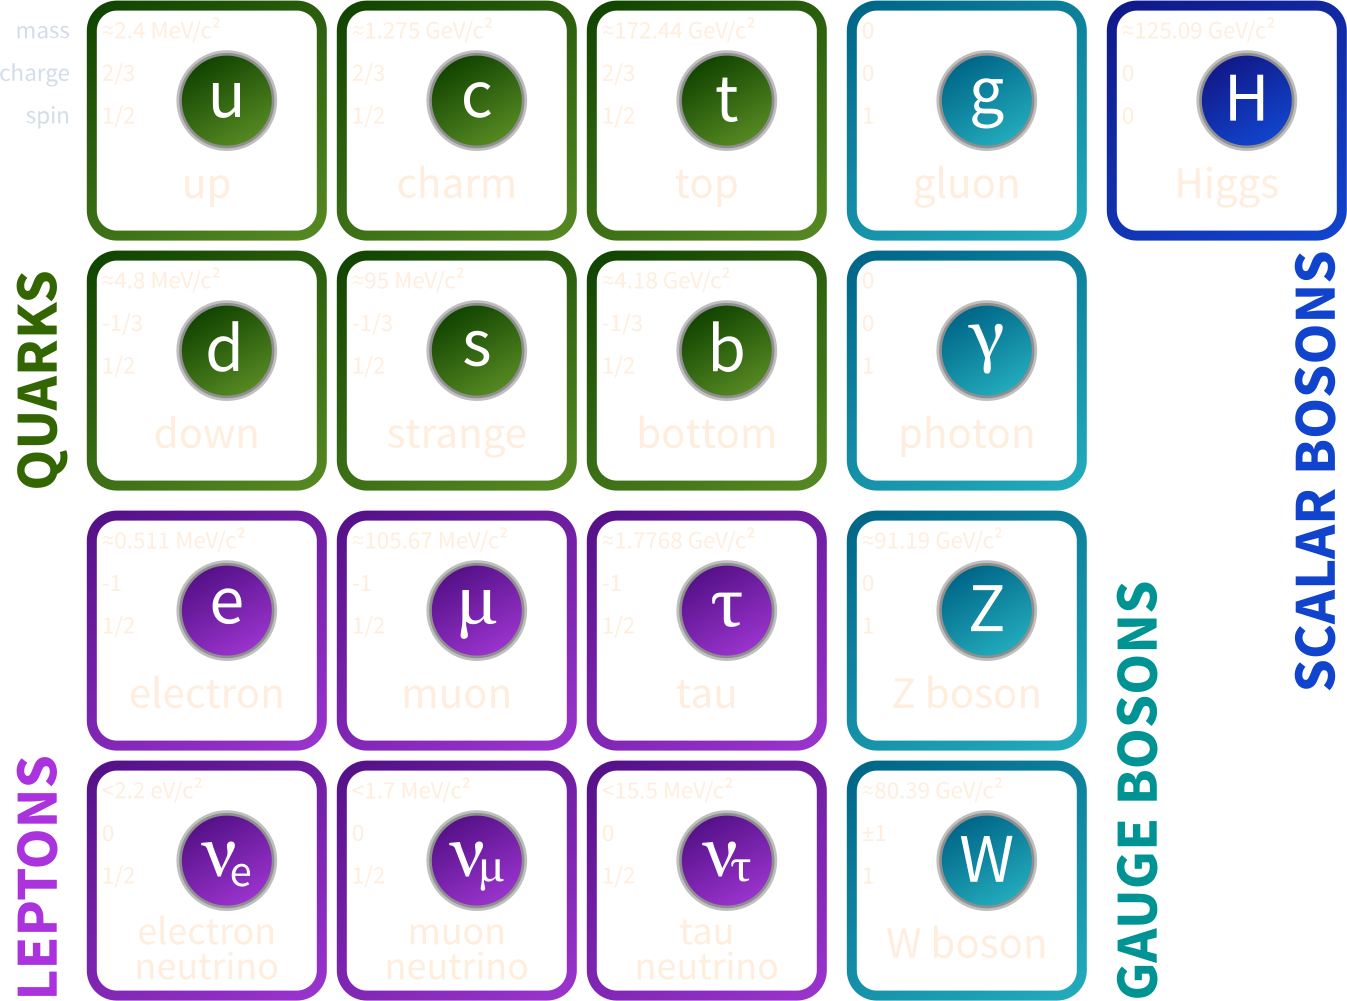
\includegraphics[width=0.7\textwidth]{particles.png}
	\end{center}
\end{frame}

\setbeamercolor{normal text}{fg=white}
\setbeamercolor{normal text}{bg=black}
\setbeamercolor{frametitle}{fg=white}
\setbeamercolor{frametitle}{bg=black}
\usebeamercolor[fg]{normal text}
\usebeamercolor[fg]{frametitle}
\usebackgroundtemplate{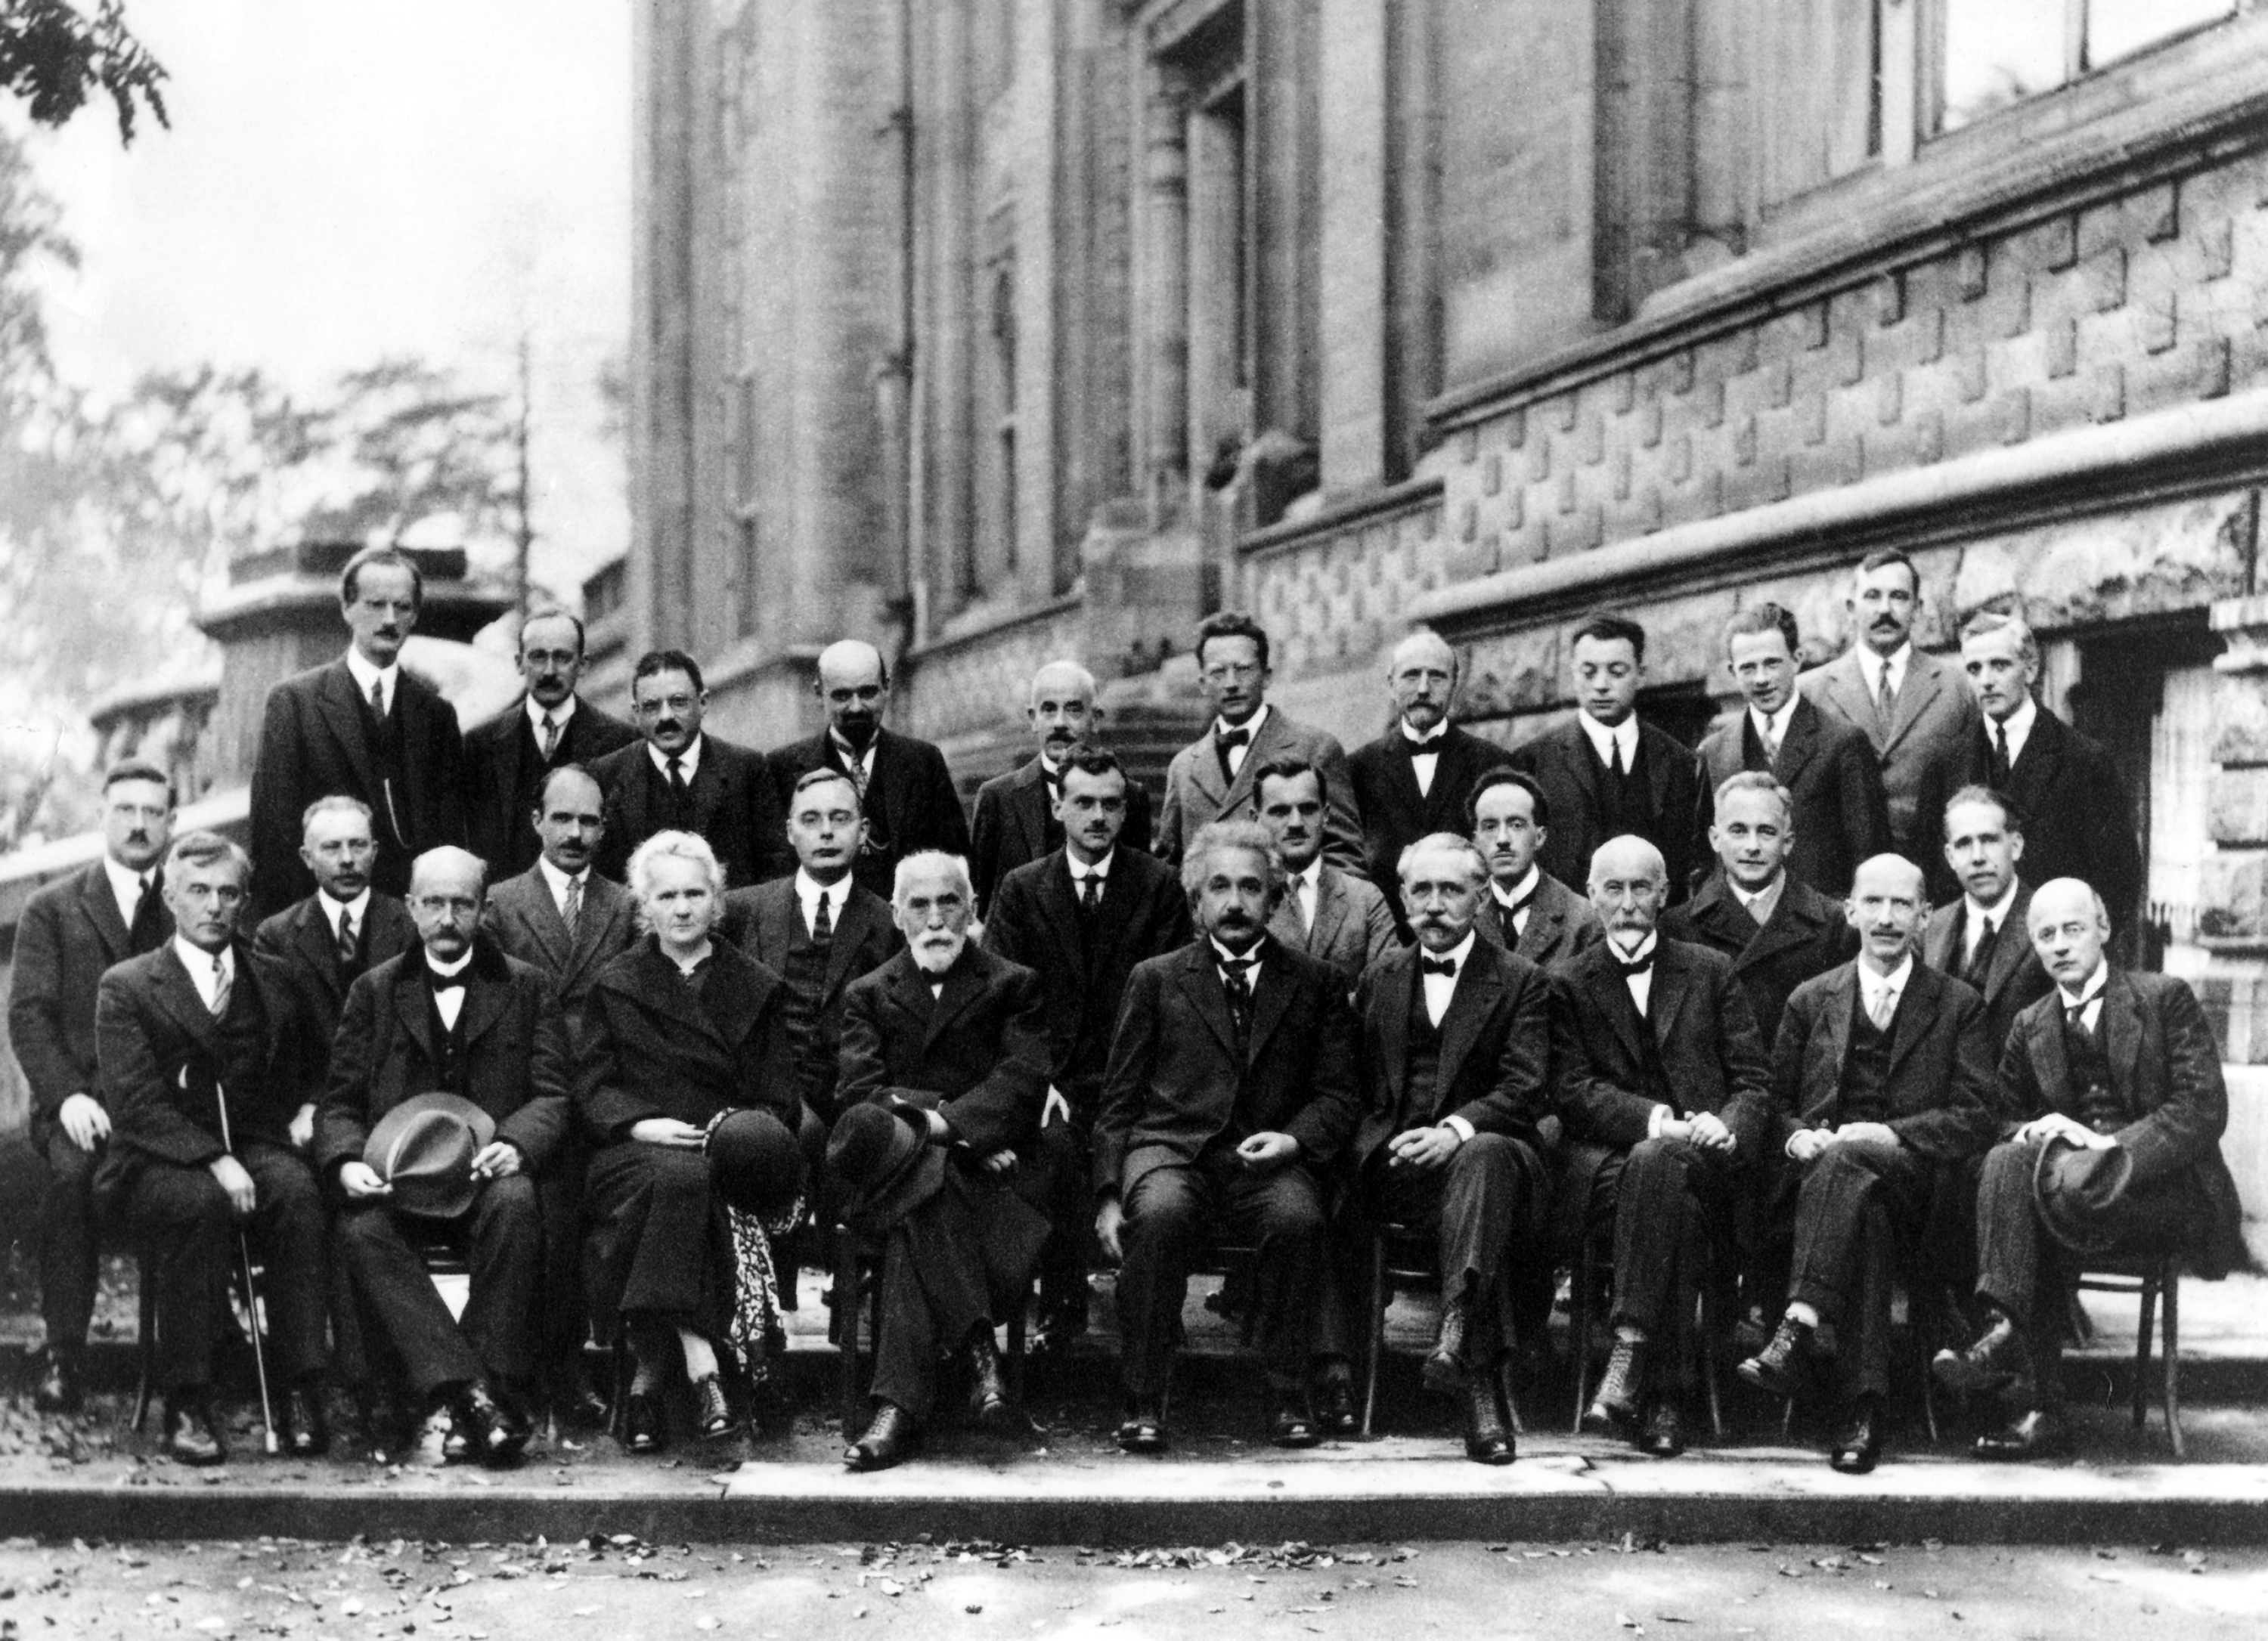
\includegraphics[width=\paperwidth]{Solvay_conference_1927.jpg}}%
\begin{frame}

\end{frame}

\begin{frame}
	\frametitle{Die wissenschaftliche Methode}
	\vspace{-1em}
	\begin{center}
		\begin{tikzpicture}[scale=6]
		\draw[draw=none](-9mm,-7mm) rectangle (9mm, 7mm);
		\arcsegment{4mm}{7mm}{65}{50}{red}{Frage}{1}
		
		\draw<1-3>[fill=black,draw=black,opacity=0.7] (0,0) circle (3.9mm);
		
		\node<1>[inner sep=0pt,align=center, text width=0.35\textwidth] (einstein) at (0,0) {    \textcolor{red}{\textit{\small Ich habe keine besondere Begabung, sondern bin nur leidenschaftlich neugierig}}\\ - \texttt{Albert Einstein}};
		
		\arcsegment{4mm}{7mm}{5}{50}{orange}{Recherche}{2}
		\node<2>[inner sep=0pt,align=center, text width=0.35\textwidth] (einstein) at (0,0) {    \textcolor{red}{\textit{Wenn ich weiter sehen konnte, so deshalb, weil ich auf den Schultern von Riesen stand.}}\\ - \texttt{Isaac Newton}};
		
		\arcsegment{4mm}{7mm}{355}{-50}{yellow}{Theorie}{3}
		\node<3>[inner sep=0pt,align=center, text width=0.37\textwidth] (einstein) at (0,0.5mm) {\small\setlength{\abovedisplayskip}{0pt}
			\setlength{\belowdisplayskip}{0pt}
			\textcolor{red}{\begin{align*}\mathcal{L} &= -1/4 F_{\mu\nu} F^{\mu\nu} \\ &+ i \bar{\psi} \slashed{D} \psi + \mathrm{h.c.} \\ &+ \psi_i y_{ij} \psi_j \phi + \mathrm{h.c.} \\ &+ |D_\mu \phi|^2 - V(\phi)\end{align*}}
			- \texttt{Standardmodell der Teilchenphysik}};
		
		\arcsegment{4mm}{7mm}{295}{-50}{green}{Experiment}{4}
		\node<4>[circle,draw=none,
		text=white,
		path picture={
			\node at (path picture bounding box.center){
				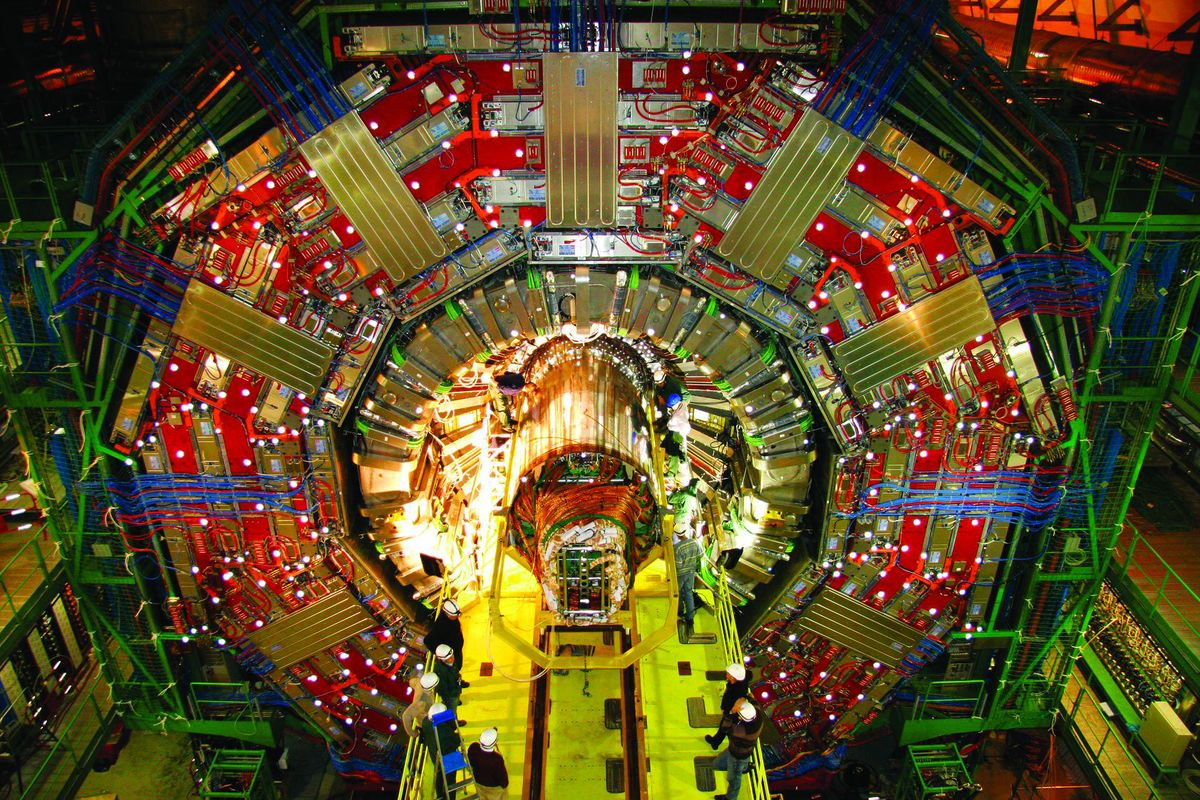
\includegraphics[width=0.6\textwidth]{cms.jpg}
			};
		}] (cms) at (0mm,0mm) {\hphantom{aaaaaaaaaaaaaaaaa}};
		
		\arcsegment{4mm}{7mm}{235}{-50}{blue}{Interpretation}{5}
		\node<5>[circle,draw=none,align=left,
		text=black,
		path picture={
			\node at (path picture bounding box.center){
				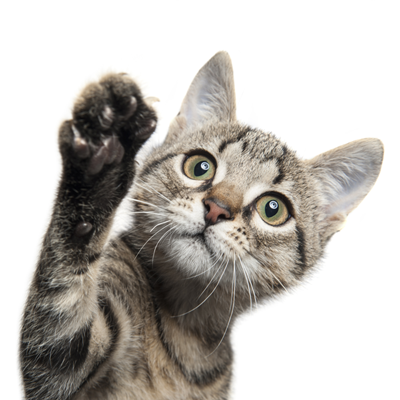
\includegraphics[width=0.4\textwidth]{katze.png}
			};
		}] (katze) at (0mm,0.1mm) {\textcolor{blue}{\hphantom{\texttt{Schröd Katze}}} \\ \\ \\ \\ };
		
		\arcsegment{4mm}{7mm}{125}{50}{purple}{Ver{\"o}ffentlichung}{6}
		\node<6>[circle,draw=none,align=left,
		text=black,
		path picture={
			\node at (path picture bounding box.center){
				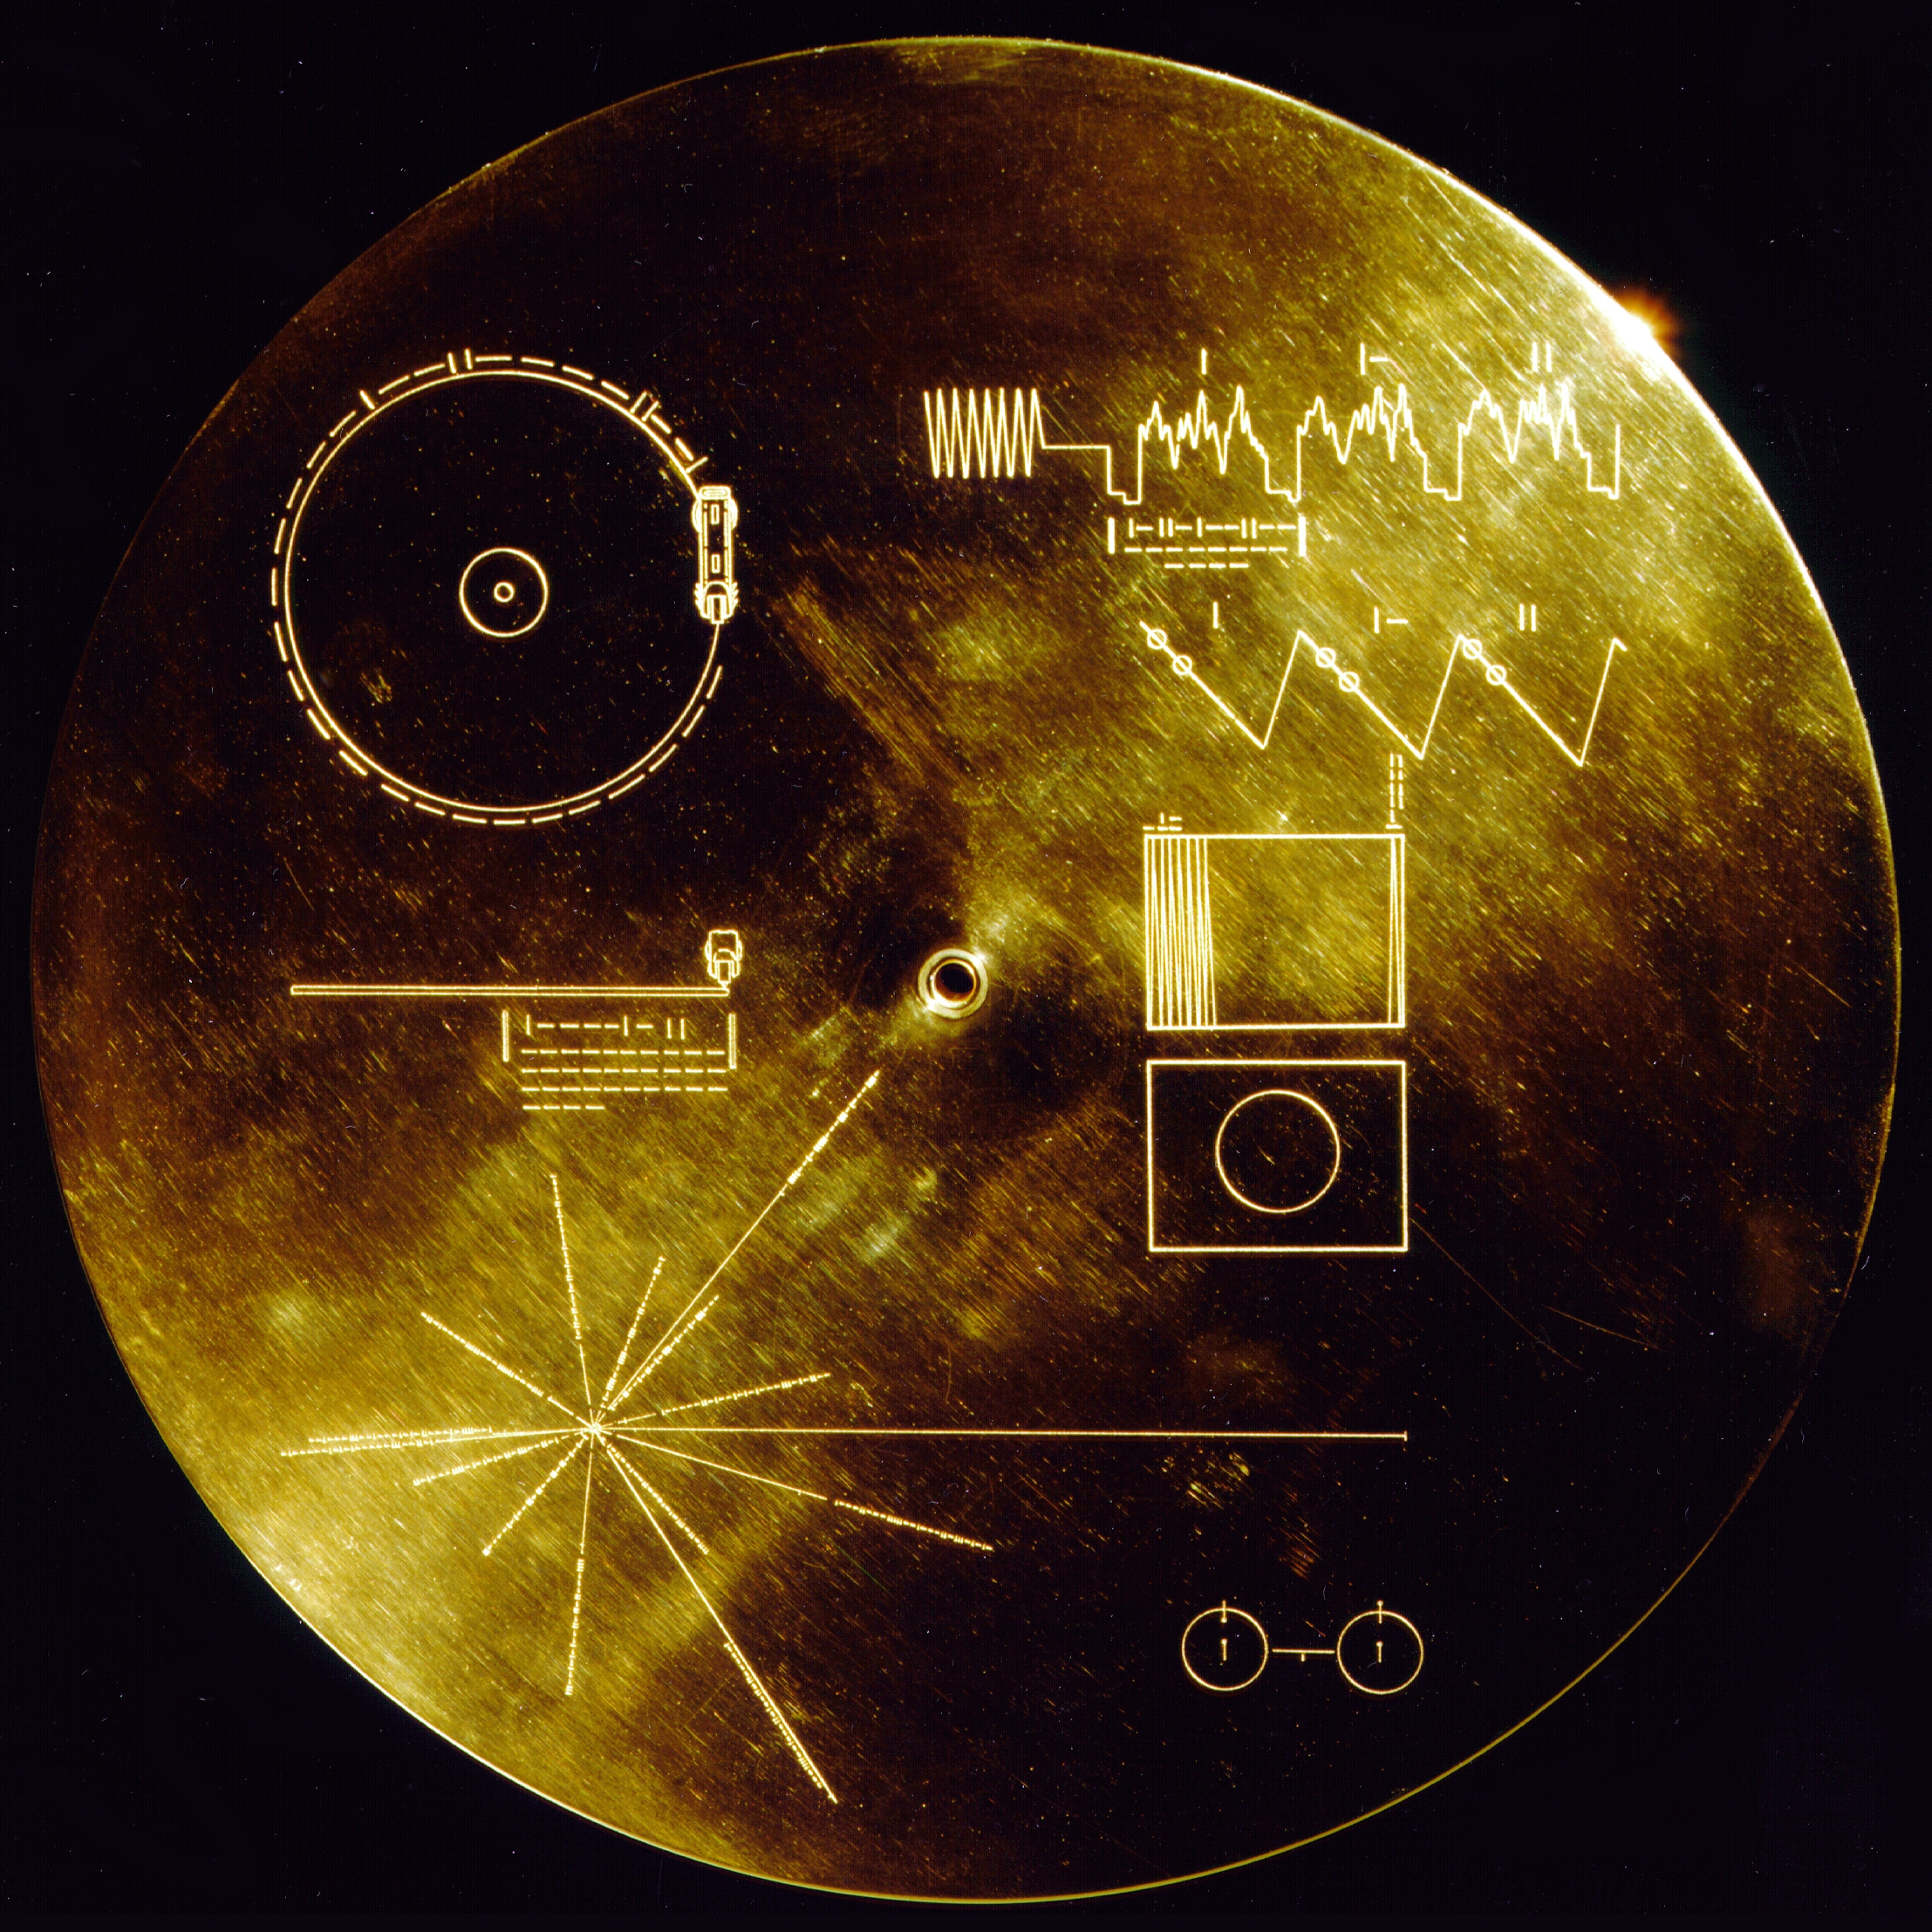
\includegraphics[width=0.42\textwidth]{voyager.jpg}
			};
		}] (voyager) at (0mm,0mm) {\textcolor{blue}{\hphantom{\texttt{Voyager Golden }}}};
		\end{tikzpicture} 
	\end{center}
\end{frame}

\usebackgroundtemplate{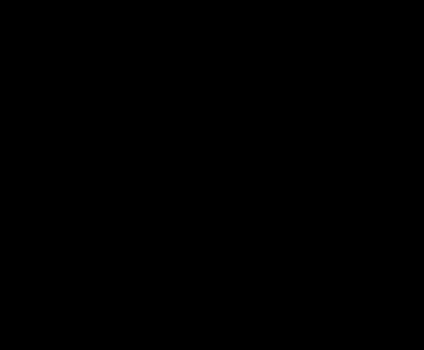
\includegraphics[width=\paperwidth]{black.png}}%

\begin{frame}
	\centering
	\large{Von der Grundlagenforschung zur Anwendung}\\
	\small{\textcolor{red}{oder}}\\
	\large{Wie funktioniert eigentlich mein Smartphone?}
\end{frame}

\begin{frame}
	\frametitle{Heinrich Hertz}
	\begin{center}
		\begin{columns}
			\begin{column}{0.5\textwidth}
		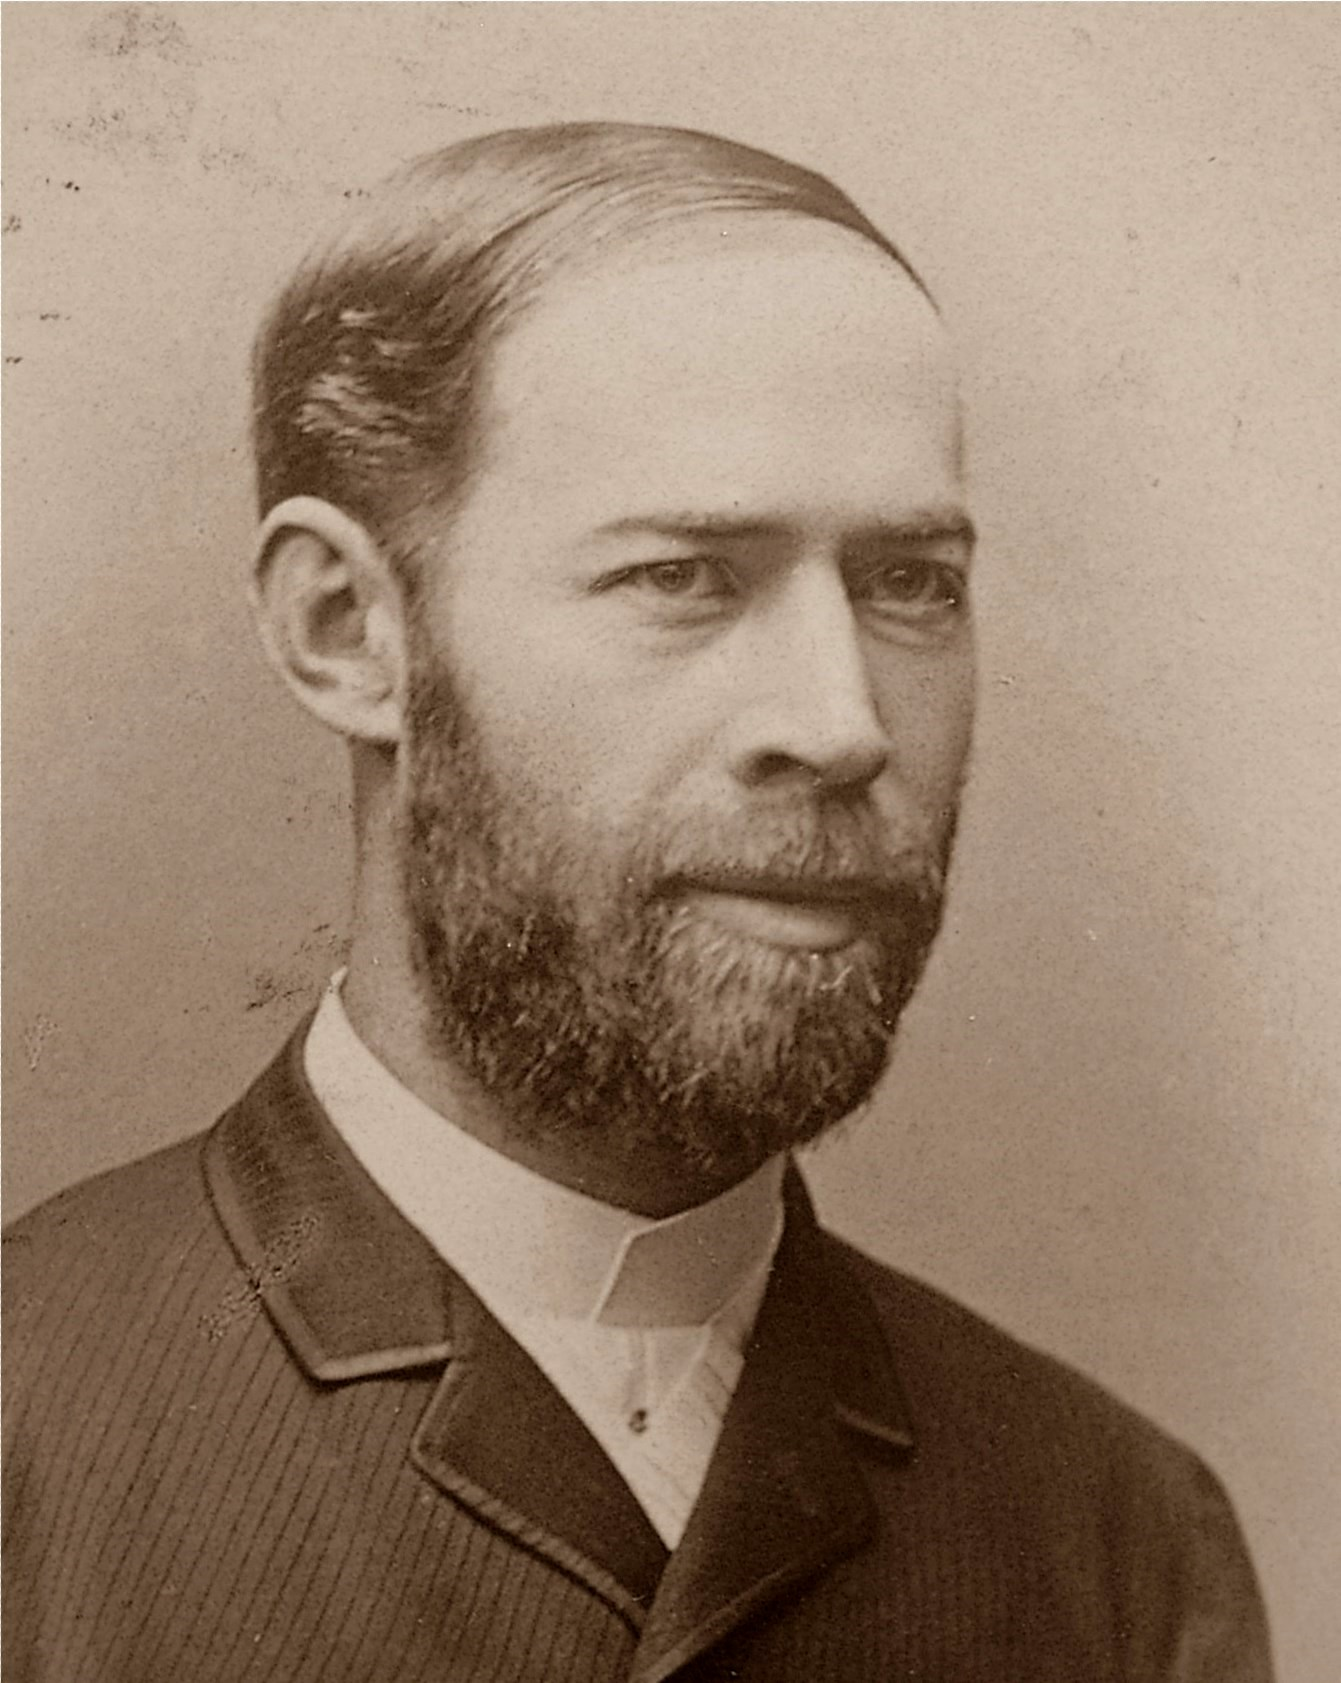
\includegraphics[width=0.9\textwidth]{heinrich_hertz.jpg}
			\end{column}
			\begin{column}{0.5\textwidth}
		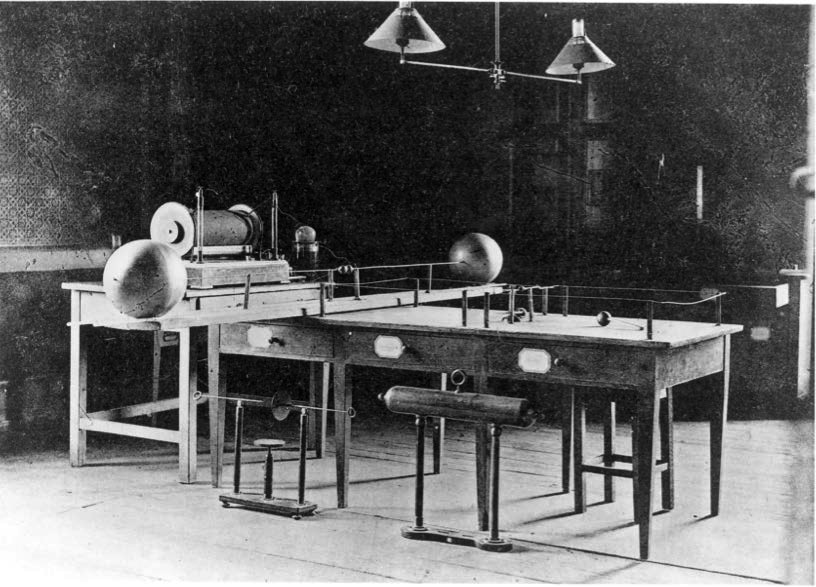
\includegraphics[width=0.9\textwidth]{heinrich_hertz_setup.jpg}
			\end{column}
		\end{columns}
		\vspace*{1em}
		\onslide<2>{WLAN, Mobilfunk}
	\end{center}
\end{frame}

\begin{frame}
	\frametitle{Otto Lehmann}
	\begin{center}
		\begin{columns}
			\begin{column}{0.5\textwidth}
		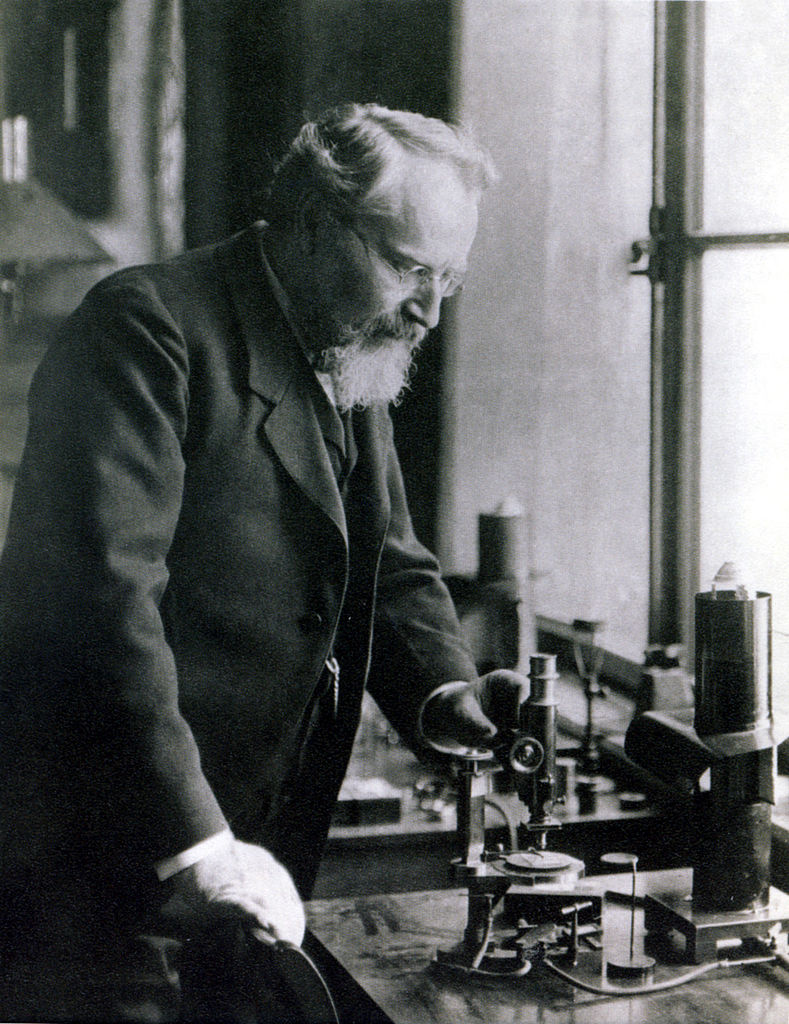
\includegraphics[width=0.9\textwidth]{otto_lehmann.jpg}
			\end{column}
			\begin{column}{0.5\textwidth}
		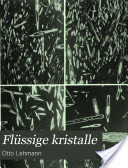
\includegraphics[width=0.9\textwidth]{otto_lehmann_book.jpg}
			\end{column}
		\end{columns}
		\vspace*{1em}
		\onslide<2>{Display}
	\end{center}
\end{frame}

\begin{frame}
	\frametitle{Albert Einstein}
	\begin{center}
		\begin{columns}
			\begin{column}{0.5\textwidth}
		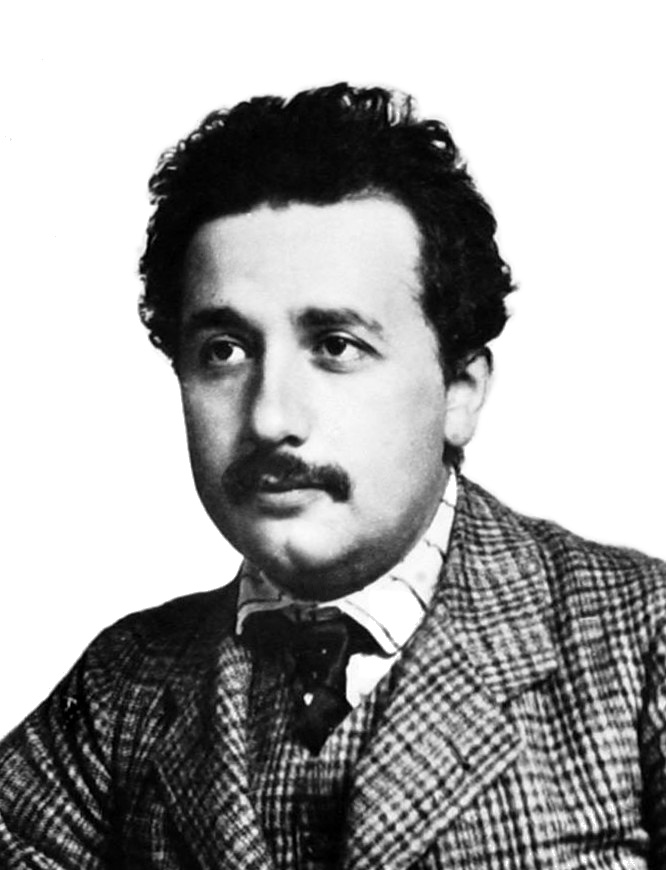
\includegraphics[width=0.9\textwidth]{albert_einstein.jpg}
			\end{column}
			\begin{column}{0.5\textwidth}
		\movie[autostart,loop,width=0.9\textwidth,height=0.4\textheight]{GPS}{gps.webm}
			\end{column}
		\end{columns}
		\vspace*{1em}
		\onslide<2>{GPS}
	\end{center}
\end{frame}

\begin{frame}
	\frametitle{John Bardeen}
	\begin{center}
		\begin{columns}
			\begin{column}{0.5\textwidth}
		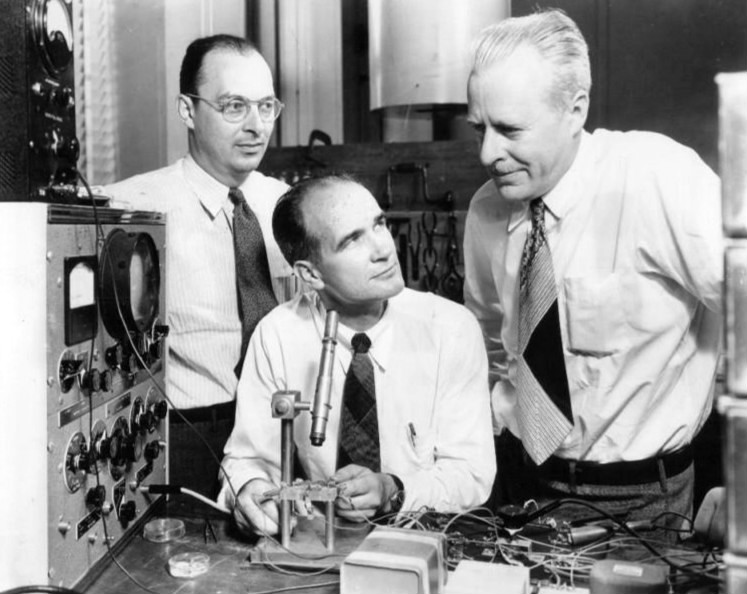
\includegraphics[width=0.9\textwidth]{john_bardeen.jpg}
			\end{column}
			\begin{column}{0.5\textwidth}
		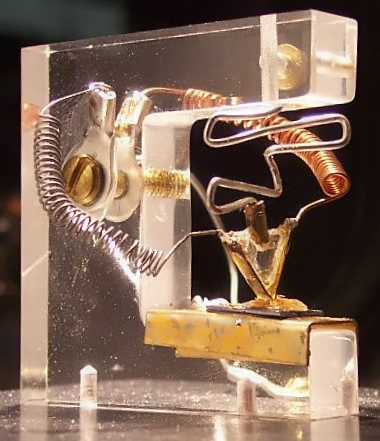
\includegraphics[width=0.9\textwidth]{john_bardeen_transistor.jpg}
			\end{column}
		\end{columns}
		
		\vspace*{1em}
		\onslide<2>{Prozessor, Elektronik}
	\end{center}
\end{frame}

\begin{frame}
	\frametitle{Tim Berners-Lee}
	\begin{center}
		\begin{columns}
			\begin{column}{0.5\textwidth}
		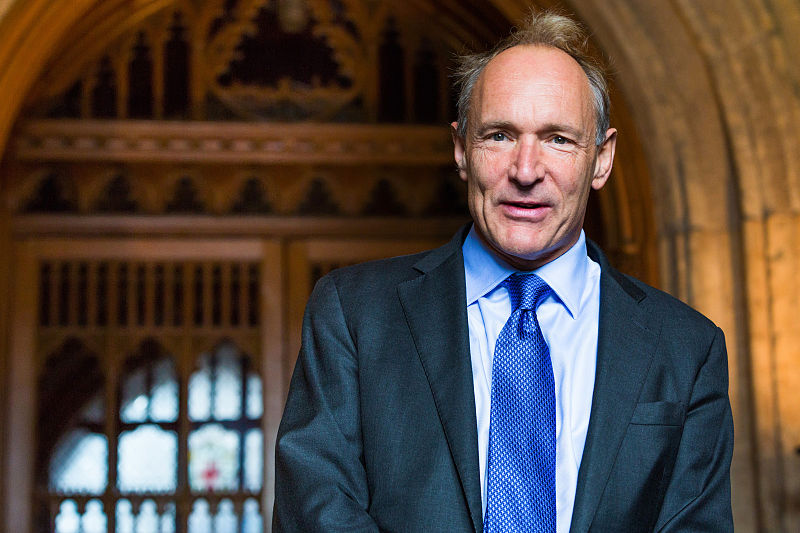
\includegraphics[width=0.9\textwidth]{tim_berners_lee.jpg}
			\end{column}
			\begin{column}{0.5\textwidth}
		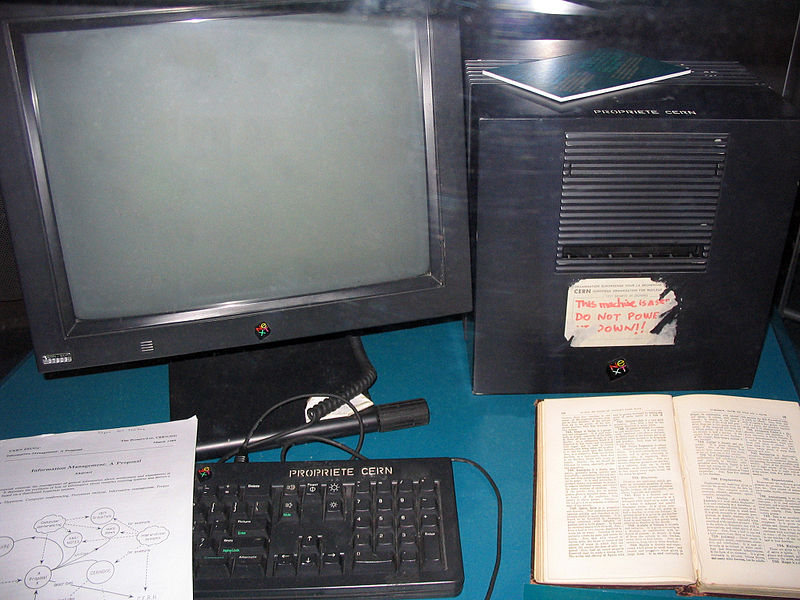
\includegraphics[width=0.9\textwidth]{tim_berners_lee_setup.jpg}
			\end{column}
		\end{columns}
		\vspace*{1em}
		\onslide<2>{World Wide Web}
	\end{center}
\end{frame}

\begin{frame}
	\frametitle{Aktuelle Revolution aus der Grundlagenforschung}
	\begin{center}
		\begin{itemize}
			\item {\large Deep Learning}
				\begin{itemize}
					\item Selbstfahrende Autos
					\item Spracherkennung
					\item Bilderkennung
					\item ,,Künstliche Intelligenz''
				\end{itemize}
			\item {\large CRISPR/Cas}
				\begin{itemize}
					\item Gentherapie
					\item Pflanzenzüchtung
					\item ,,Gen-Bomben''
				\end{itemize}
		\end{itemize}
	\end{center}
\end{frame}

\begin{frame}
	
	\vspace{2em}
	\begingroup
	\advance\leftmargini -2.6em
	\begin{quote}
		Ich weiß nicht, für was das einmal gut sein wird.\\ Aber ich weiß, dass Sie Steuern darauf nehmen werden.\\ -- \texttt{Michael Faraday}
	\end{quote}
	\endgroup
\end{frame}
	
\end{document}
